\documentclass[dvipdfmx,a4paper,12pt]{jsarticle}

\title{M輪講 Factoring integers}
\author{252305012~~~伊藤 碧己}

\usepackage[dvipdfmx]{graphicx}

\begin{document}
\maketitle


\begin{figure}[htbp]
  \centering
  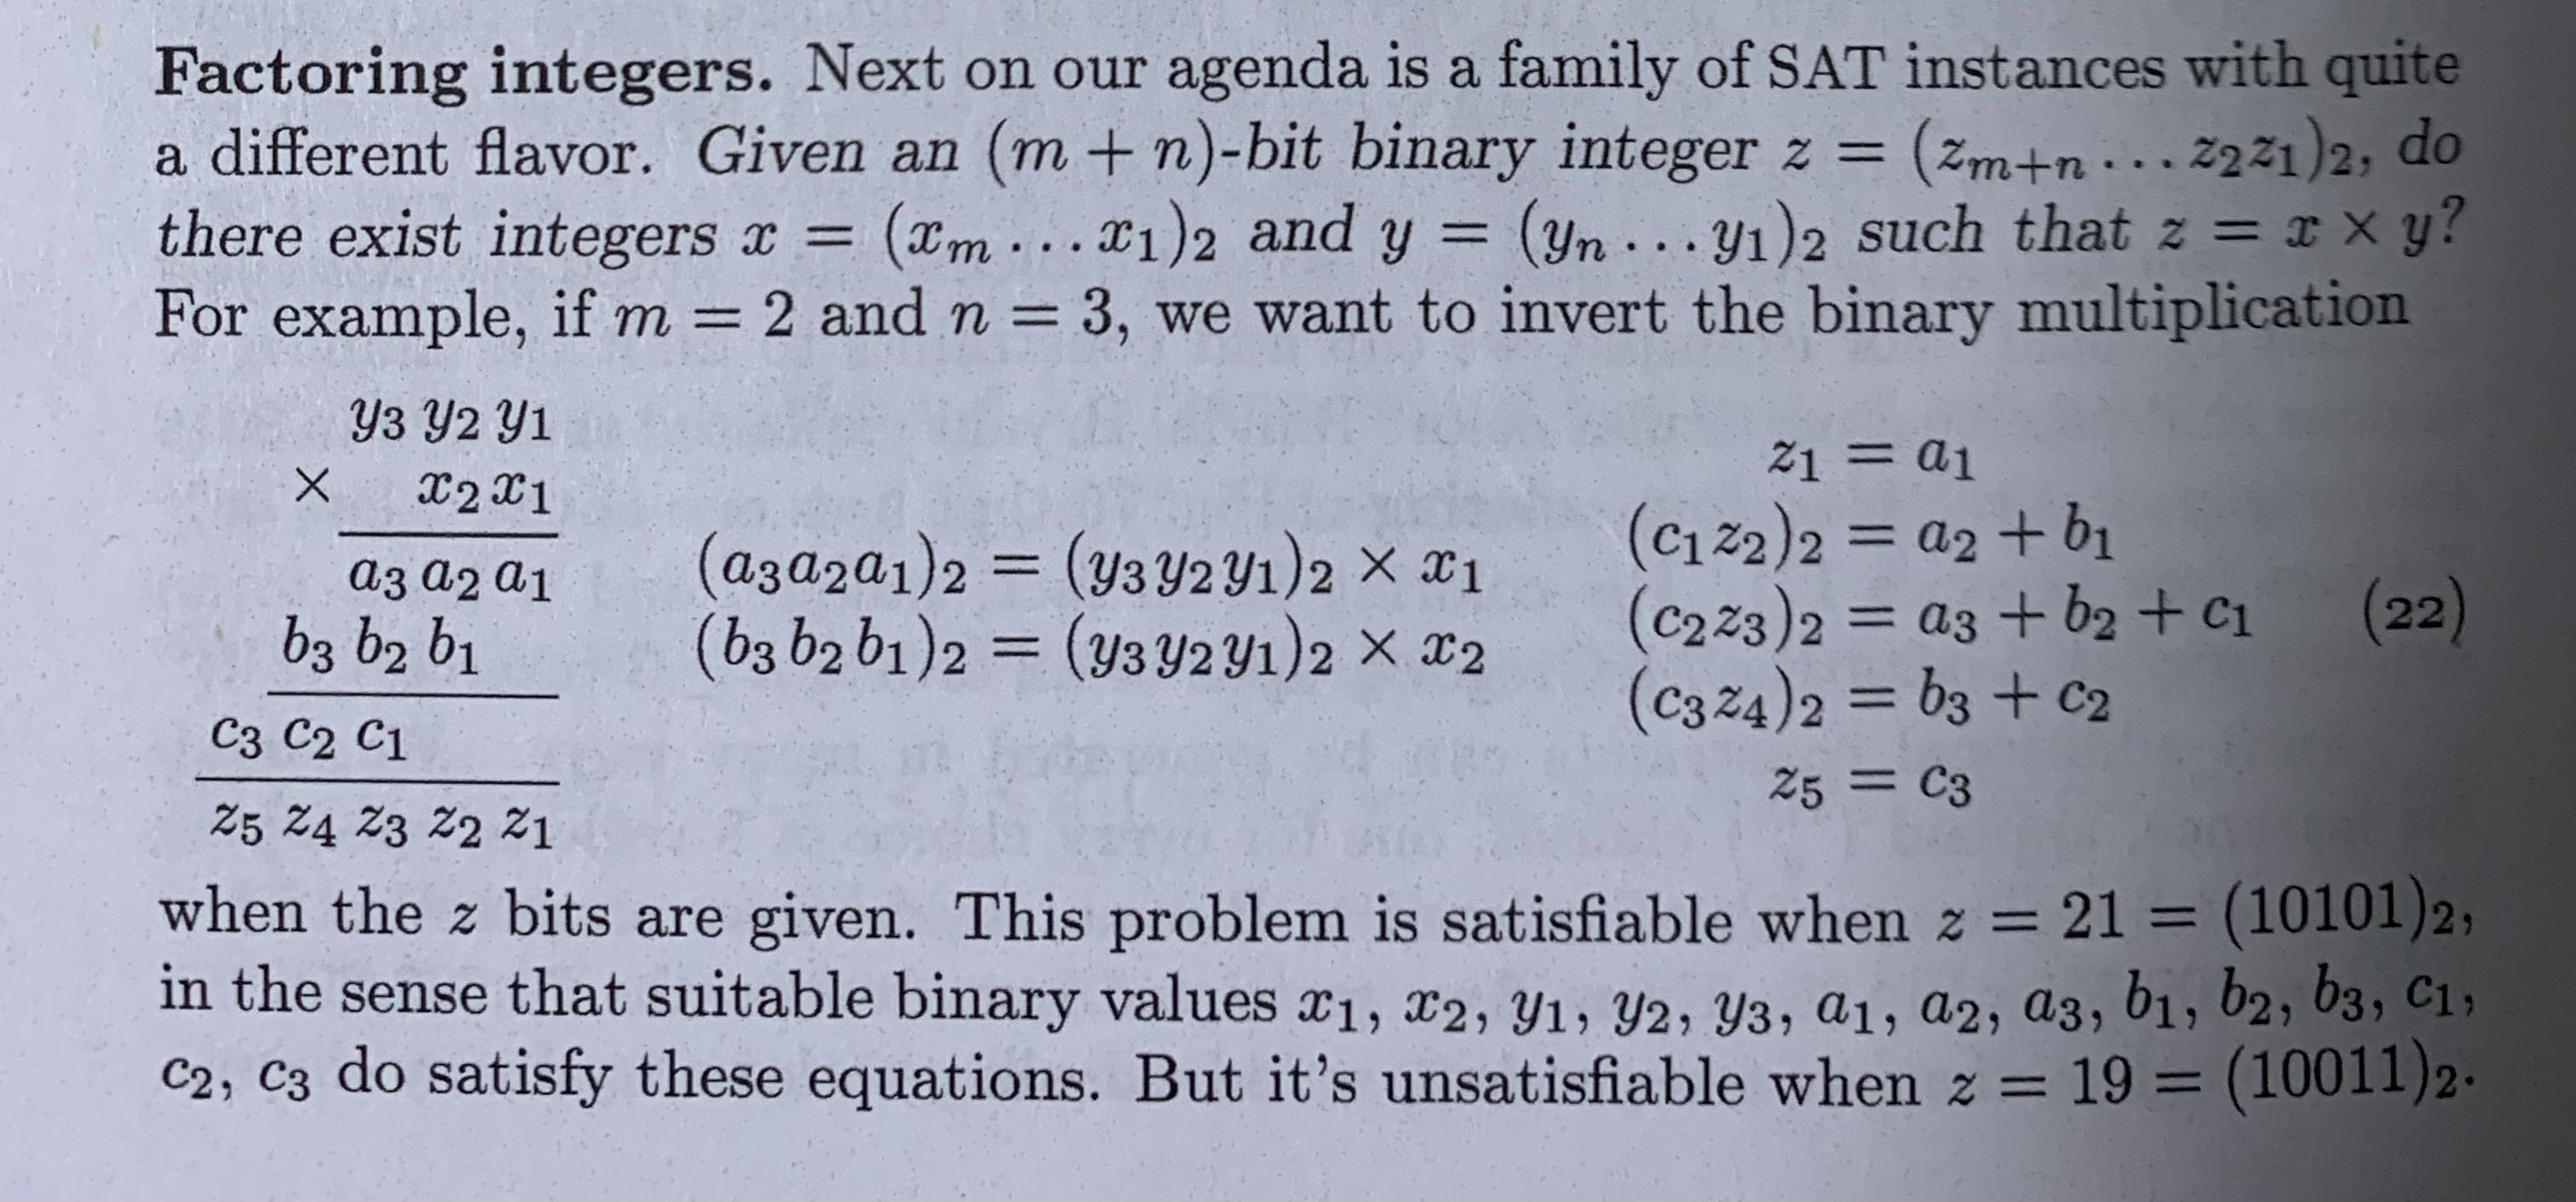
\includegraphics[width=130mm]{images/IMG_7379.jpg}
\end{figure}

因数分解. 次のテーマは,まったく異なったテイストのSATインスタンスファミリーである.$(m+n)$bitの2進整数$z=(z_{m+n}...z_{2}z_{1})_{2}$が与えれた時,そのような整数$x=(x_{m}...x_{1})_{2}$,$y=(y_{n}...y_{1})_{2}$は存在するだろうか,$z=x×y$となる.例えば,m=2,n=3の時,2進数の乗算を転換させたい.\footnote{乗算の形から因数分解を考えるという意味?}zビット\footnote{即ち2進整数z}が与えられた時.この問題は$z=21=(10101)_{2}$の時充足される,適切な2進数$x_{1},x_{2},y_{1},y_{2},y_{3},a_{1},a_{2},a_{3},b_{1},b_{2},b_{3},c_{1},c_{2},c_{3}$がこれらの等式\footnote{(22)の等式}を満たすという意味で.\footnote{$x=(11)_{2},y=7(111)_{2}すなわちa_{1}=1,a_{2}=1,a_{3}=1,b_{1}=1,b_{2}=1,b_{3}=1,c_{1}=1,c_{2}=1,c_{3}=1,z_{1}=1,z_{2}=0,z_{3}=1,z_{4}=0,z_{5}=1$}
しかし,$z=19=(10011)_{2}$のときは充足不能である.
%%%%%%%%%%%%%%%%%%%%%%%%%
\newpage
\begin{figure}[htbp]
  \centering
  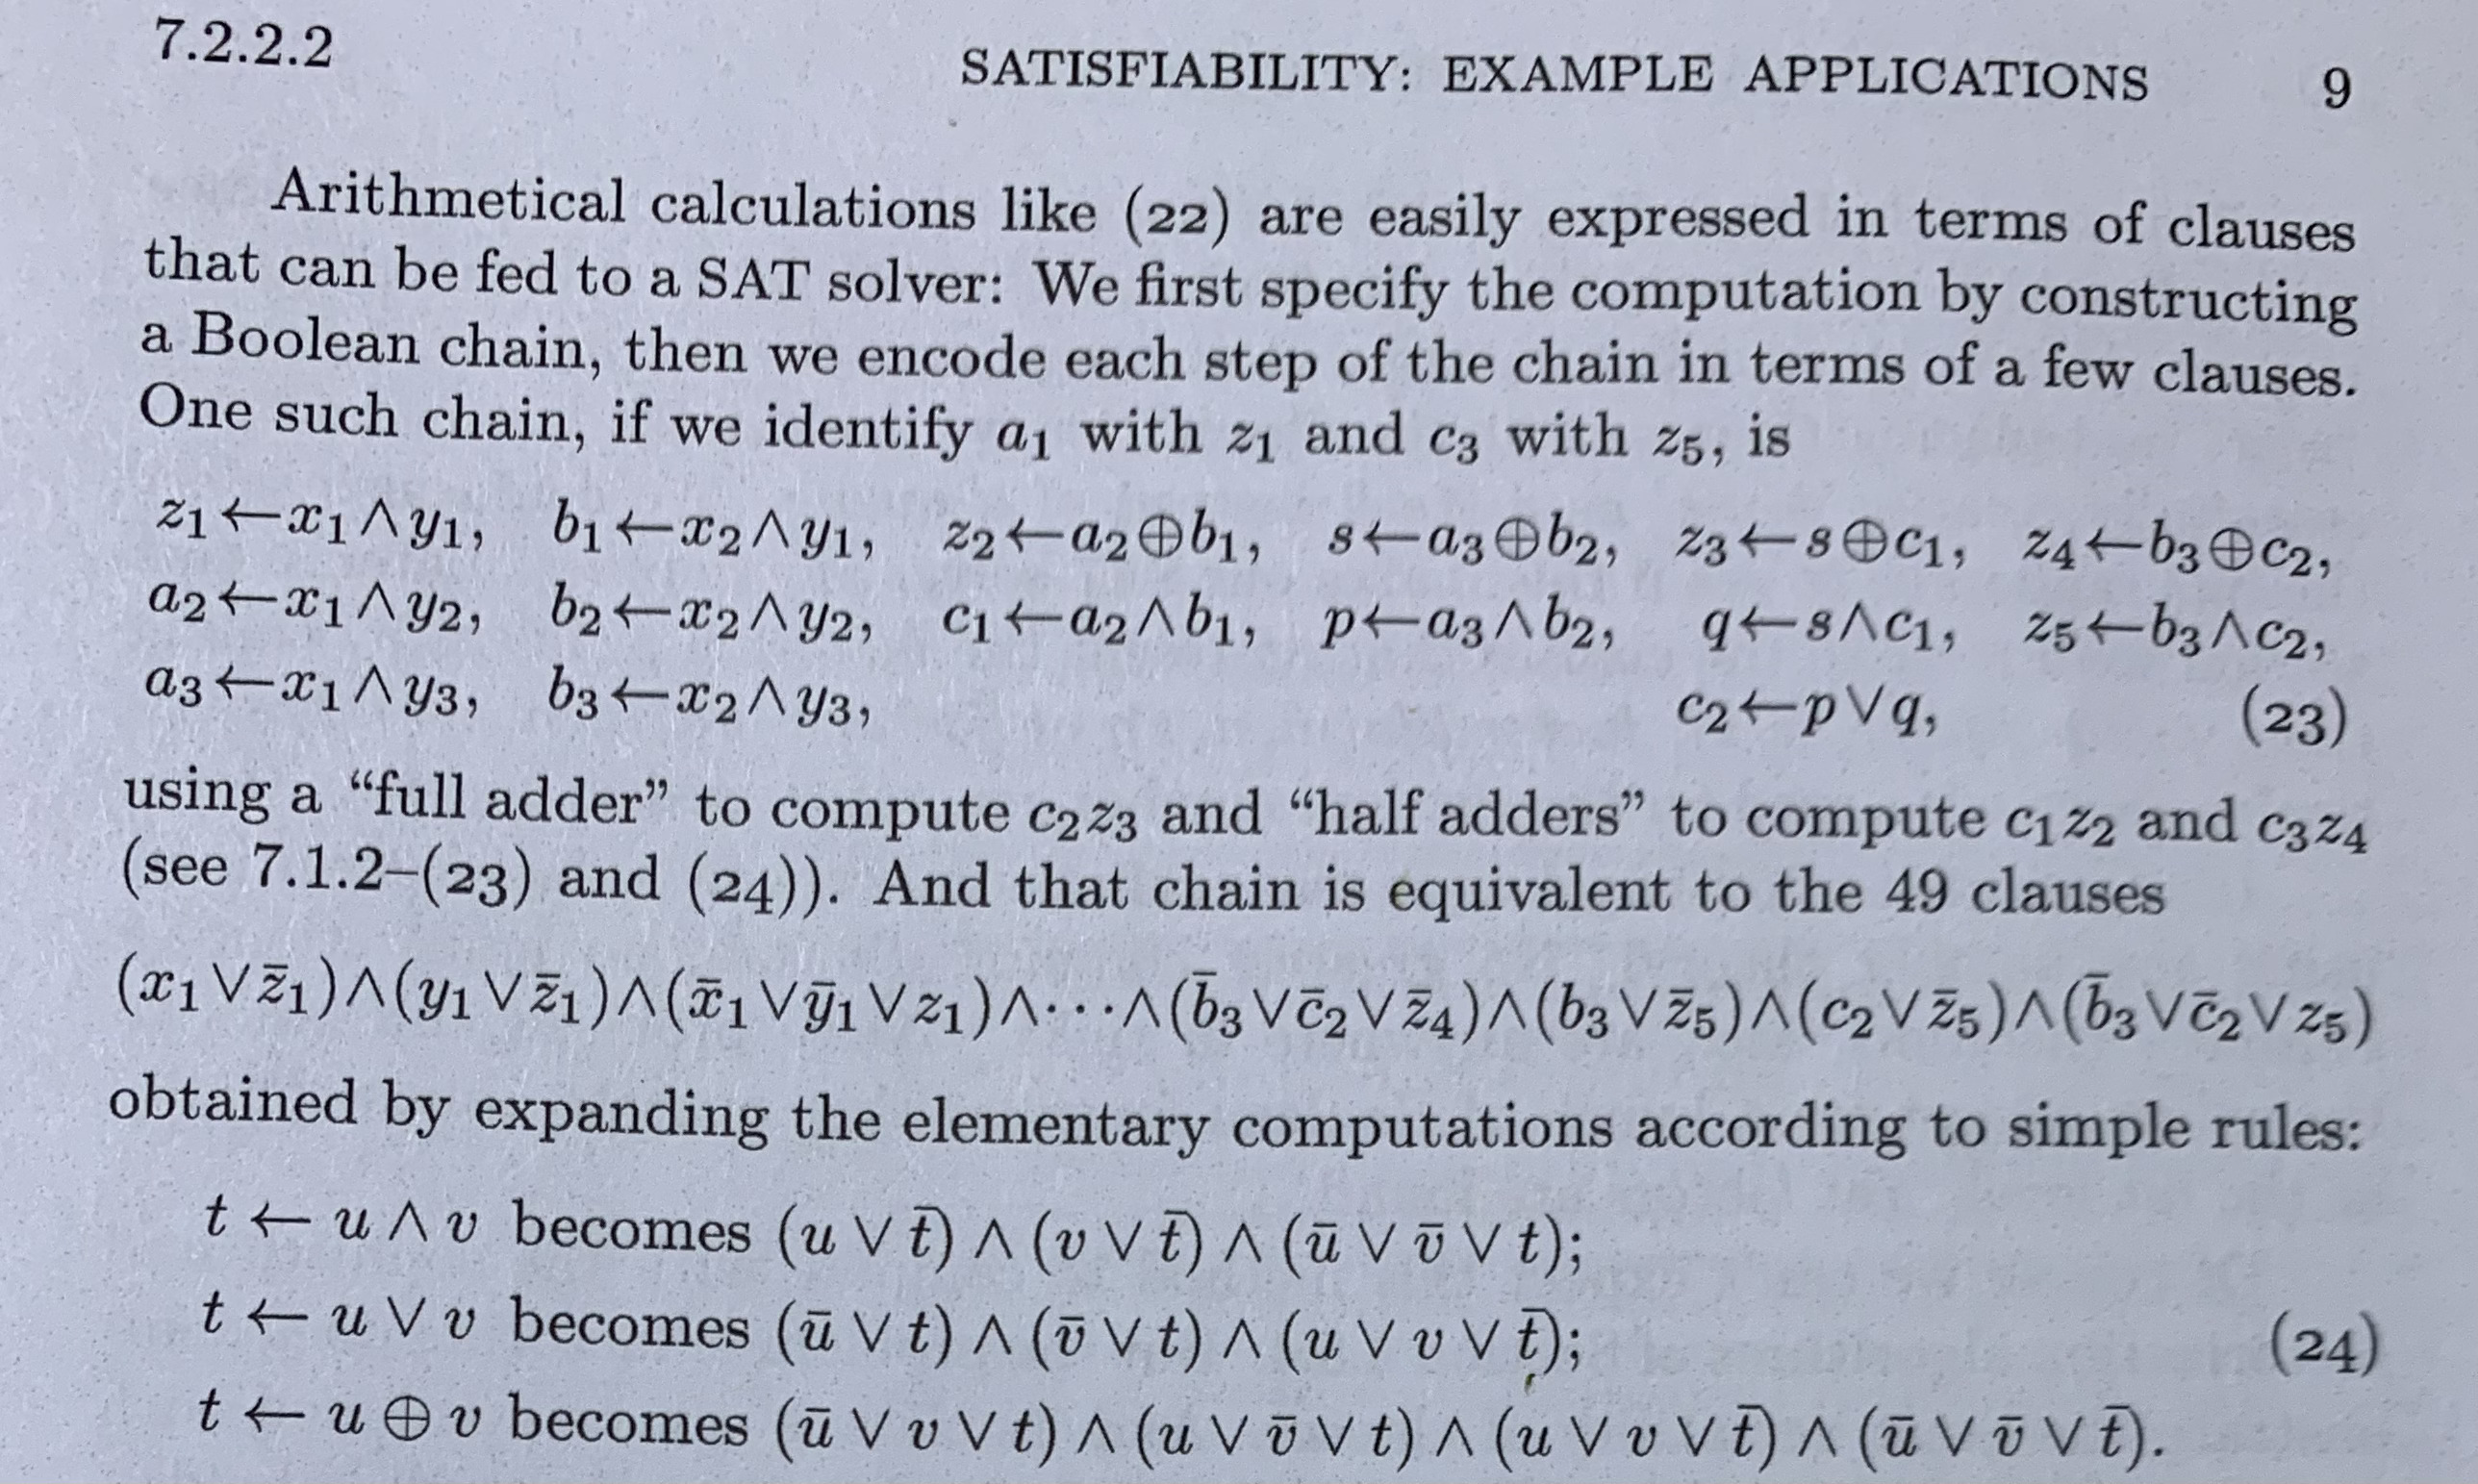
\includegraphics[width=130mm]{images/IMG_7380.jpg}
\end{figure}
(22)のような算術的な計算は,SATソルバーに与えることができる節として簡単に表現することができる: まず,ブール鎖\footnote{ブール代数において、複数の真偽値を論理演算子でつないで一つの式として表したもの}を構築することによってその計算を明記し,その鎖の各ステップをいくつかの節で符号化する.
そのような鎖の1つは,$a_{1}$を$z_{1}$,$c_{3}$を$z_{5}$とすると,$c_{2}z_{3}$の計算に「全加算器」を,$c_{1}z_{2}$と$c_{3}z_{4}$の計算に「半加算器」を使用している(7.1.2-(23),(24)を参照).
そしてその鎖は49の節$(x_{1}\vee \bar{z}_{1})\wedge(y_{1}\vee \bar{z}_{1})\wedge ... \wedge (\bar{b}_{3}\vee \bar{c}_{2} \vee z_{5})$と同値である,簡単なルール(24)で基礎的な計算を拡張することによって得られる.\footnote{(24)のルールは,「←」を同値の記号「$\leftrightarrow$」と置き換えて考えれば理解しやすい} \footnote{$\oplus$...XOR(排他的論理和)} \footnote{$A\oplus B = \bar{A} \cdot B+A\cdot \bar{B}$}
%%%%%%%%%%%%%%%%%%%%%%%%%
\newpage
\begin{figure}[htbp]
  \centering
  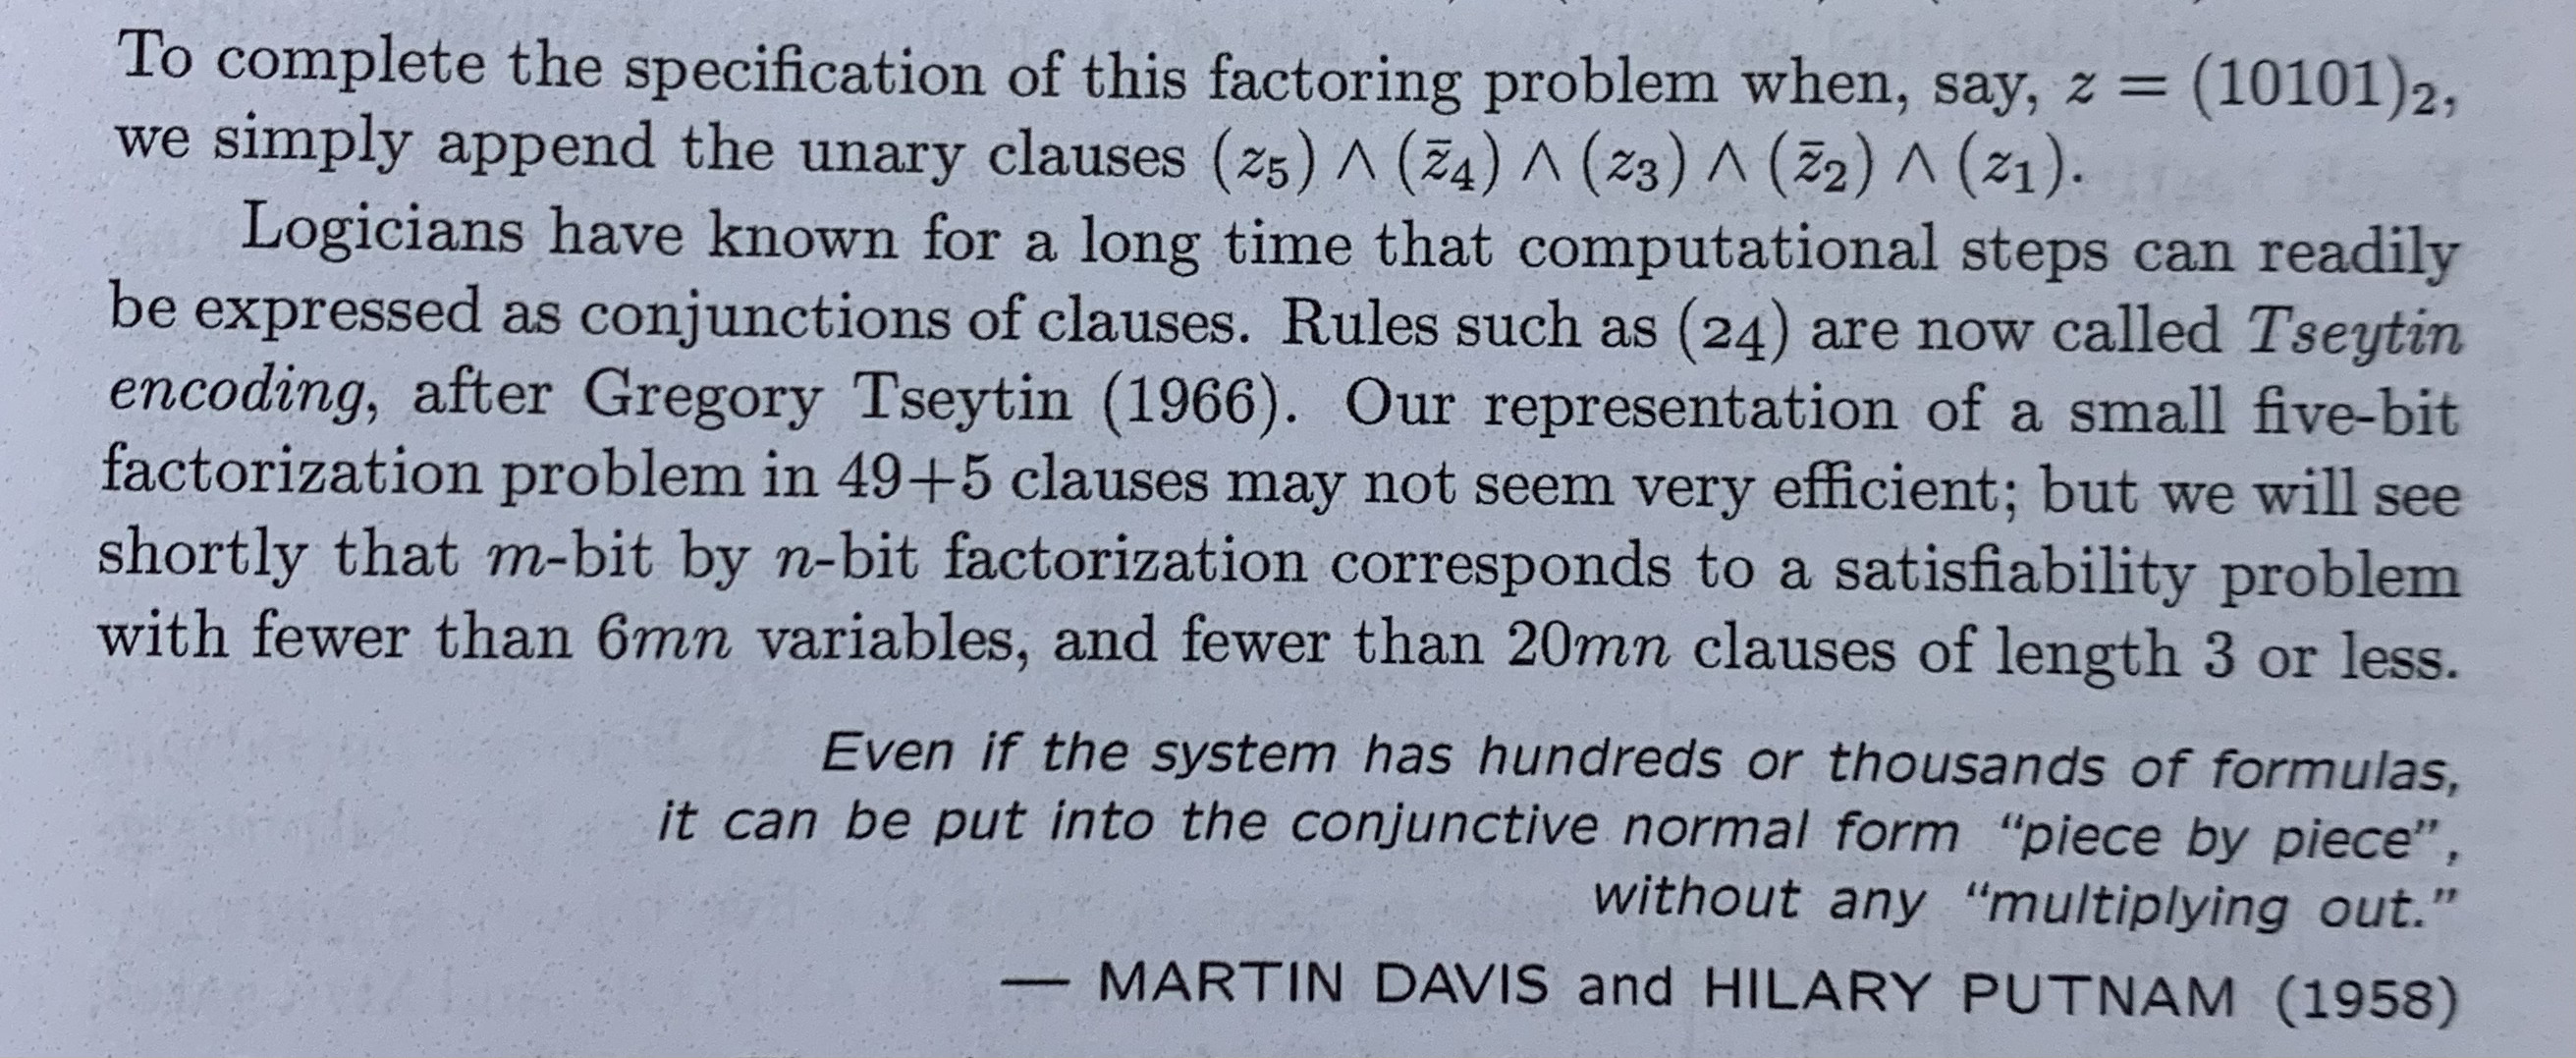
\includegraphics[width=130mm]{images/IMG_73802.jpg}
\end{figure}

この因数分解問題の仕様を完成させるために,例えば,$z=(10101)_{2}$のとき,単に単位節$z_{5}\wedge \bar{z}_{4} \wedge z_{3} \wedge \bar{z}_{2} \wedge z_{1}$を追加する.\\
論理学者たちは,長い間知っていた,計算ステップが節の連結として容易に表現できることを.(24)のようなルールはは現在,Tseytin変換と呼ばれている,Gregory Tseytin(1966)\footnote{Gregory Tseytin(1936-2022):ロシアの数学者およびコンピューター科学者.Tseitin変換の生みの親}にちなんで.5ビットの小さな因数分解問題を49 + 5の節で表現したのは,あまり効率的ではないかもしれない; しかし,まもなく分かる,mビット×nビットの因数分解はSAT問題に対応する,$6mn$以下の変数と$20mn$以下の長さ3以下の節の.\\
---たとえ数百,数千の式を持つシステムでも,"1つ1つ"連言標準形に落とし込むことができる,拡大することなく---\\
--- MARTIN DAVIS\footnote{Martin Davis(1928-2023): アメリカの数学者およびコンピューター科学者.DPLLアルゴリズムの共同開発者} and HILARY PUTNAM\footnote{Hilary Putnam(1926-2016):スコットランドの哲学者およびコンピューター科学者.DPLLアルゴリズムの共同開発者}(1958)

%%%%%%%%%%%%%%%%%%%%%%%%%
\newpage
\begin{figure}[htbp]
  \centering
  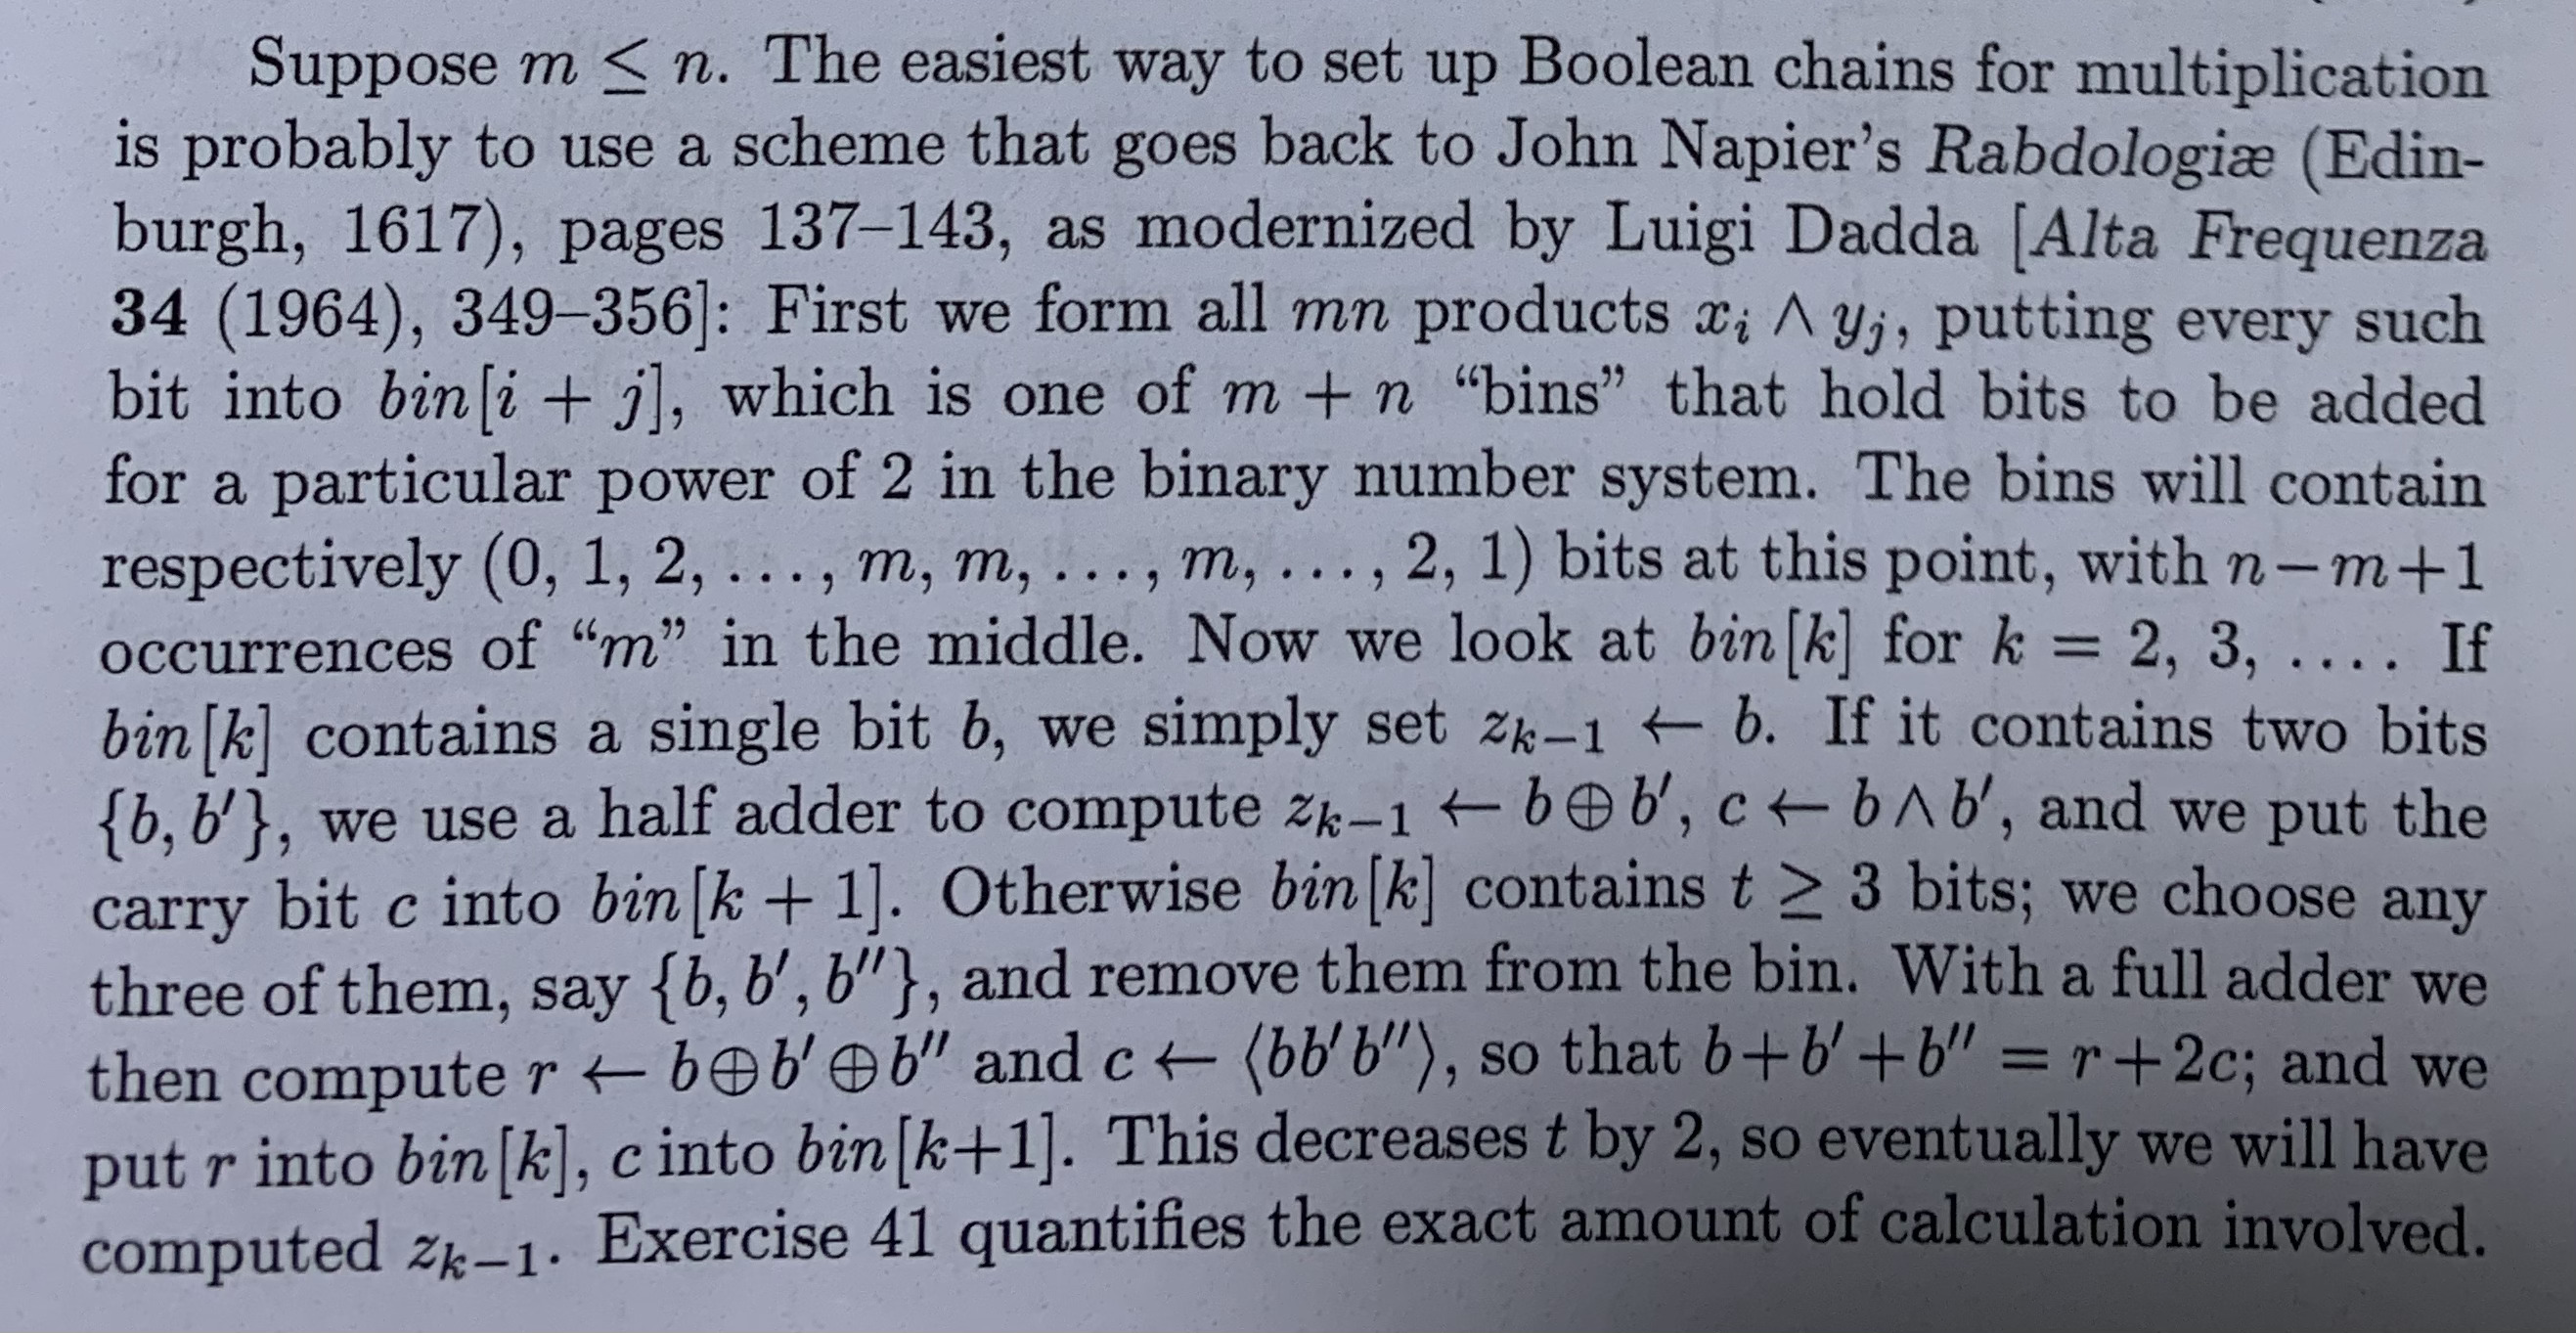
\includegraphics[width=130mm]{images/IMG_73803.jpg}
\end{figure}
$m \leq n$とする.掛け算のブール鎖を用意する最も簡単な方法はおそらく,John Napier\footnote{John Napier(1550-1617):スコットランドの数学者.対数を考案した}の \textit{Rabdologi\ae} (Edin-burgh, 1617)\footnote{1617年エディンバラで出版されたJohn Napierのラブドロジーという論文.算術計算を支援する 3 つの装置について説明している}に遡る方式を使うことだろう,その137-143ページをLuigi Daddaによって現代風にアレンジされたもの [Alta Frequenza 34 (1964), 349-356]として: まず,mn個の積$x_{i} \wedge y_{j}$をすべて形成し,そのような全てのビットをbin[i + j]に格納する.これはm + n個の「ビン」の1つである,2進数システムの特定の2のべき乗に対して追加されるビットを保持する.ビンは,この時点でそれぞれ(0,1,2,...,m,m,...,2,1)ビットを含み,真ん中ではn-m+1回の"m"が出現する.ここで,k = 2, 3, ...の場合のbin [k]を確認する.もし
bin [k]に1つのビットbが含まれている場合,単に$z_{k-1} ← b$をセットし,2つのビット\{b, b'\}が含まれている場合は,半加算器で$z_{k-1}←b \oplus b'$, $c←b\wedge b'$を計算し,キャリービットcをbin [k + 1] に入れる.それ以外の場合,bin[k]には$t\geq 3$ビットが含まれる.そのうちの任意の3つ,例えば\{b,b', b''\}を選び,ビンから削除する.そして全加算器によって$r← b \oplus b' \oplus b''$と$c←〈bb'b''〉$\footnote{〈〉の意味は調べてもわからなかった.計算の意味を考えると〈〉の中のブール変数のうち2つ以上が真なら真と考察できる}を計算すると,b+b' +b" = r + 2cとなるので\footnote{r+2cの2cというのは,2進数で1つ上の桁にcを足すことを意味している(memo)},rをbin[k]に、cをbin[k+1]に入れる.これでtが2減るので,最終的には$z_{k-1}$を計算したことになる.練習問題41は,正確な計算量を数値化したものある.
\newpage
\begin{figure}[htbp]
  \centering
  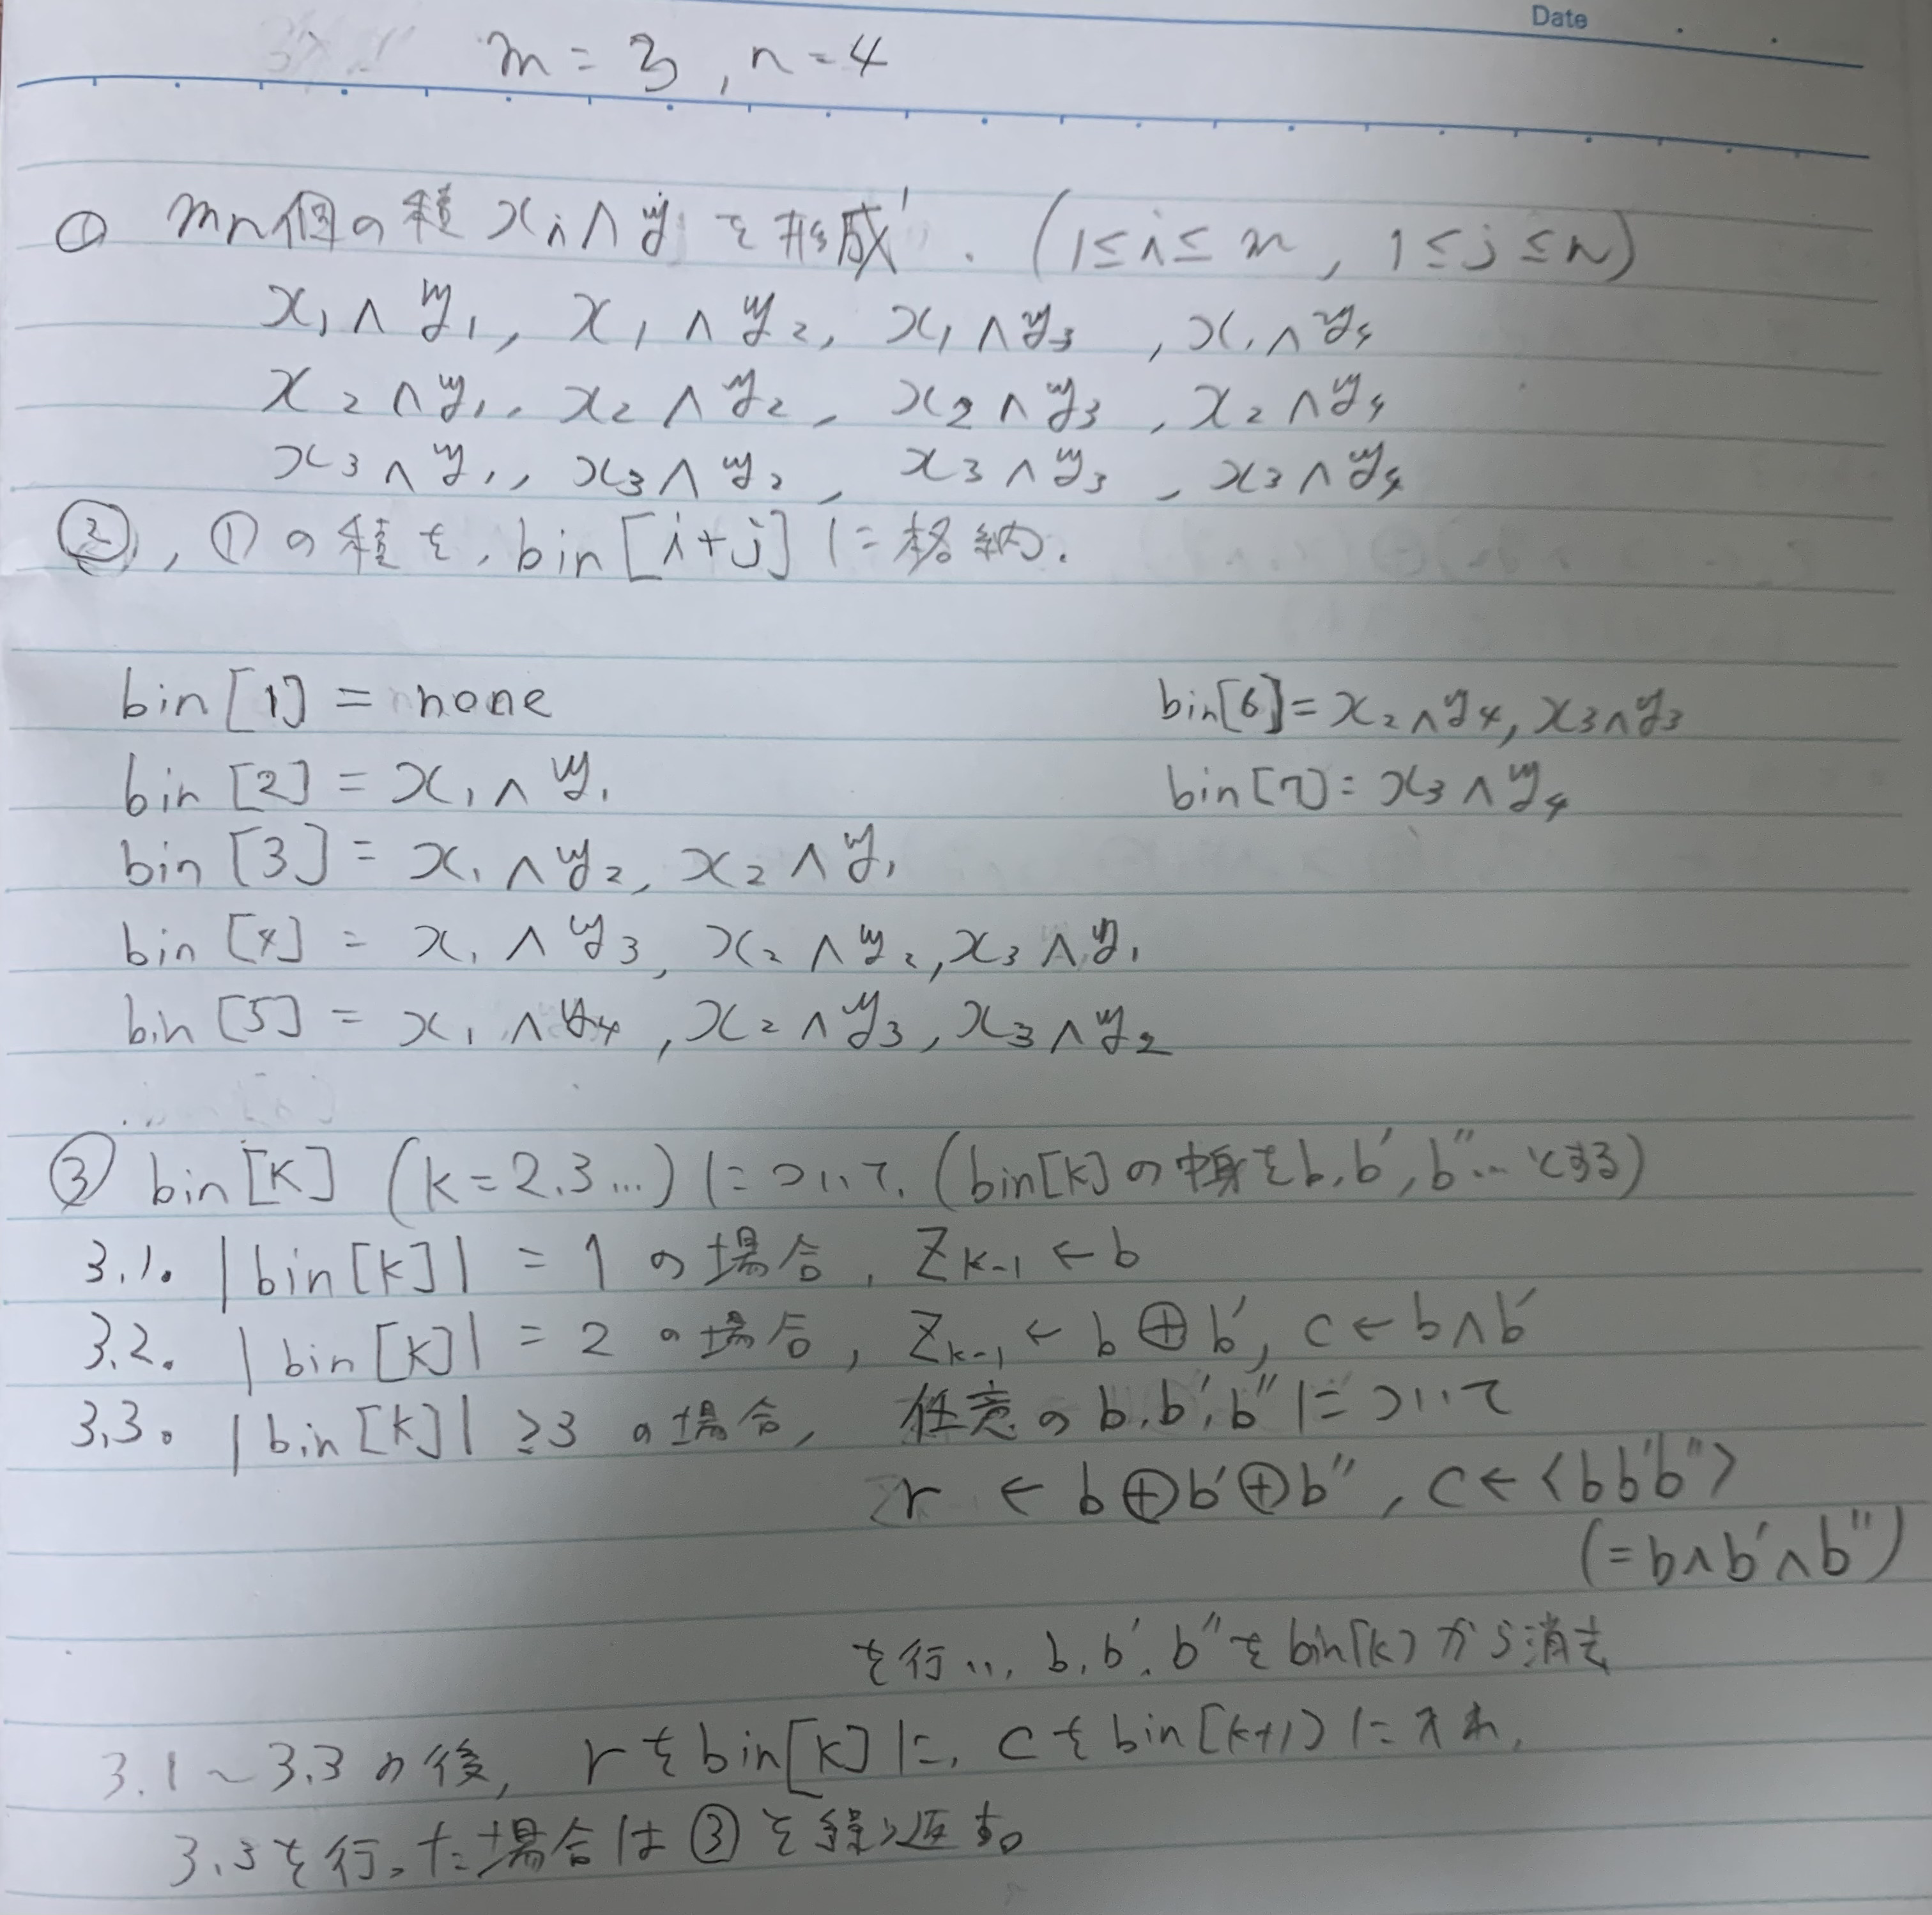
\includegraphics[width=130mm]{images/IMG_7410.jpg}
  \caption{計算の例(m=3,n=4)}
\end{figure}

\newpage
\begin{figure}[htbp]
  \centering
  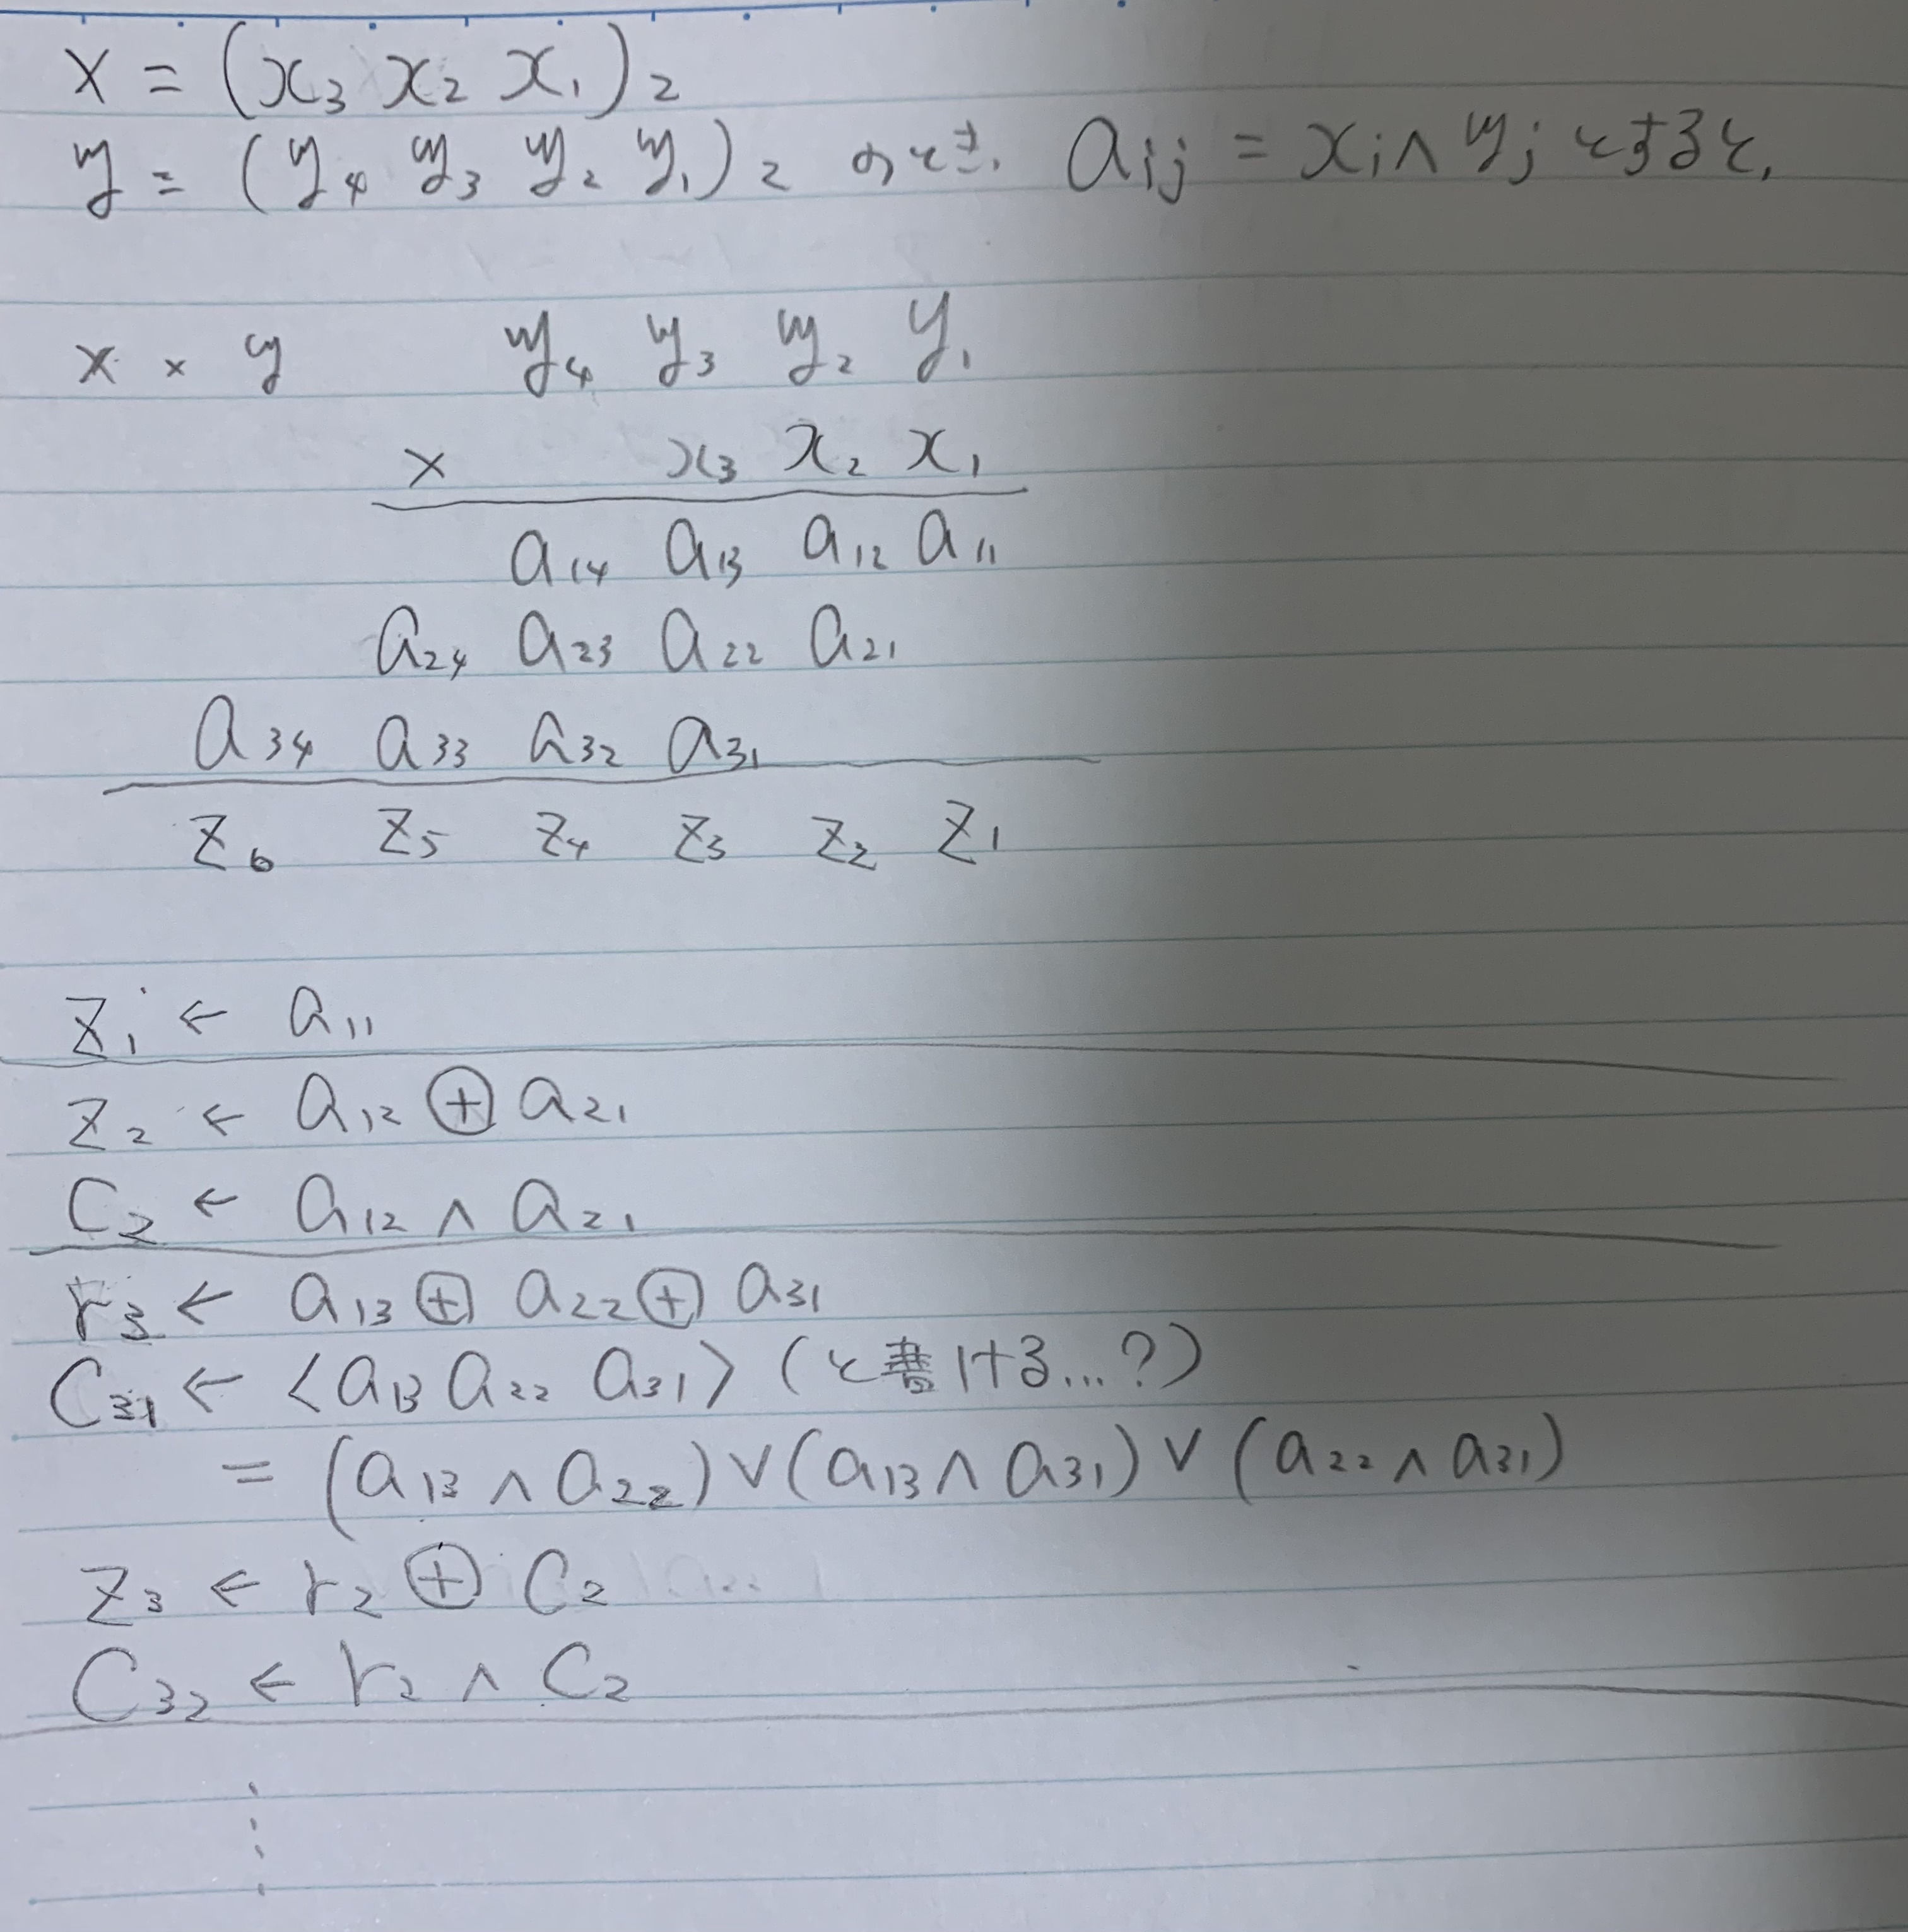
\includegraphics[width=130mm]{images/IMG_7409.jpg}
  \caption{計算例:ステップ3}
\end{figure}
%%%%%%%%%%%%%%%%%%%%%%%%%
\newpage
\begin{figure}[htbp]
  \centering
  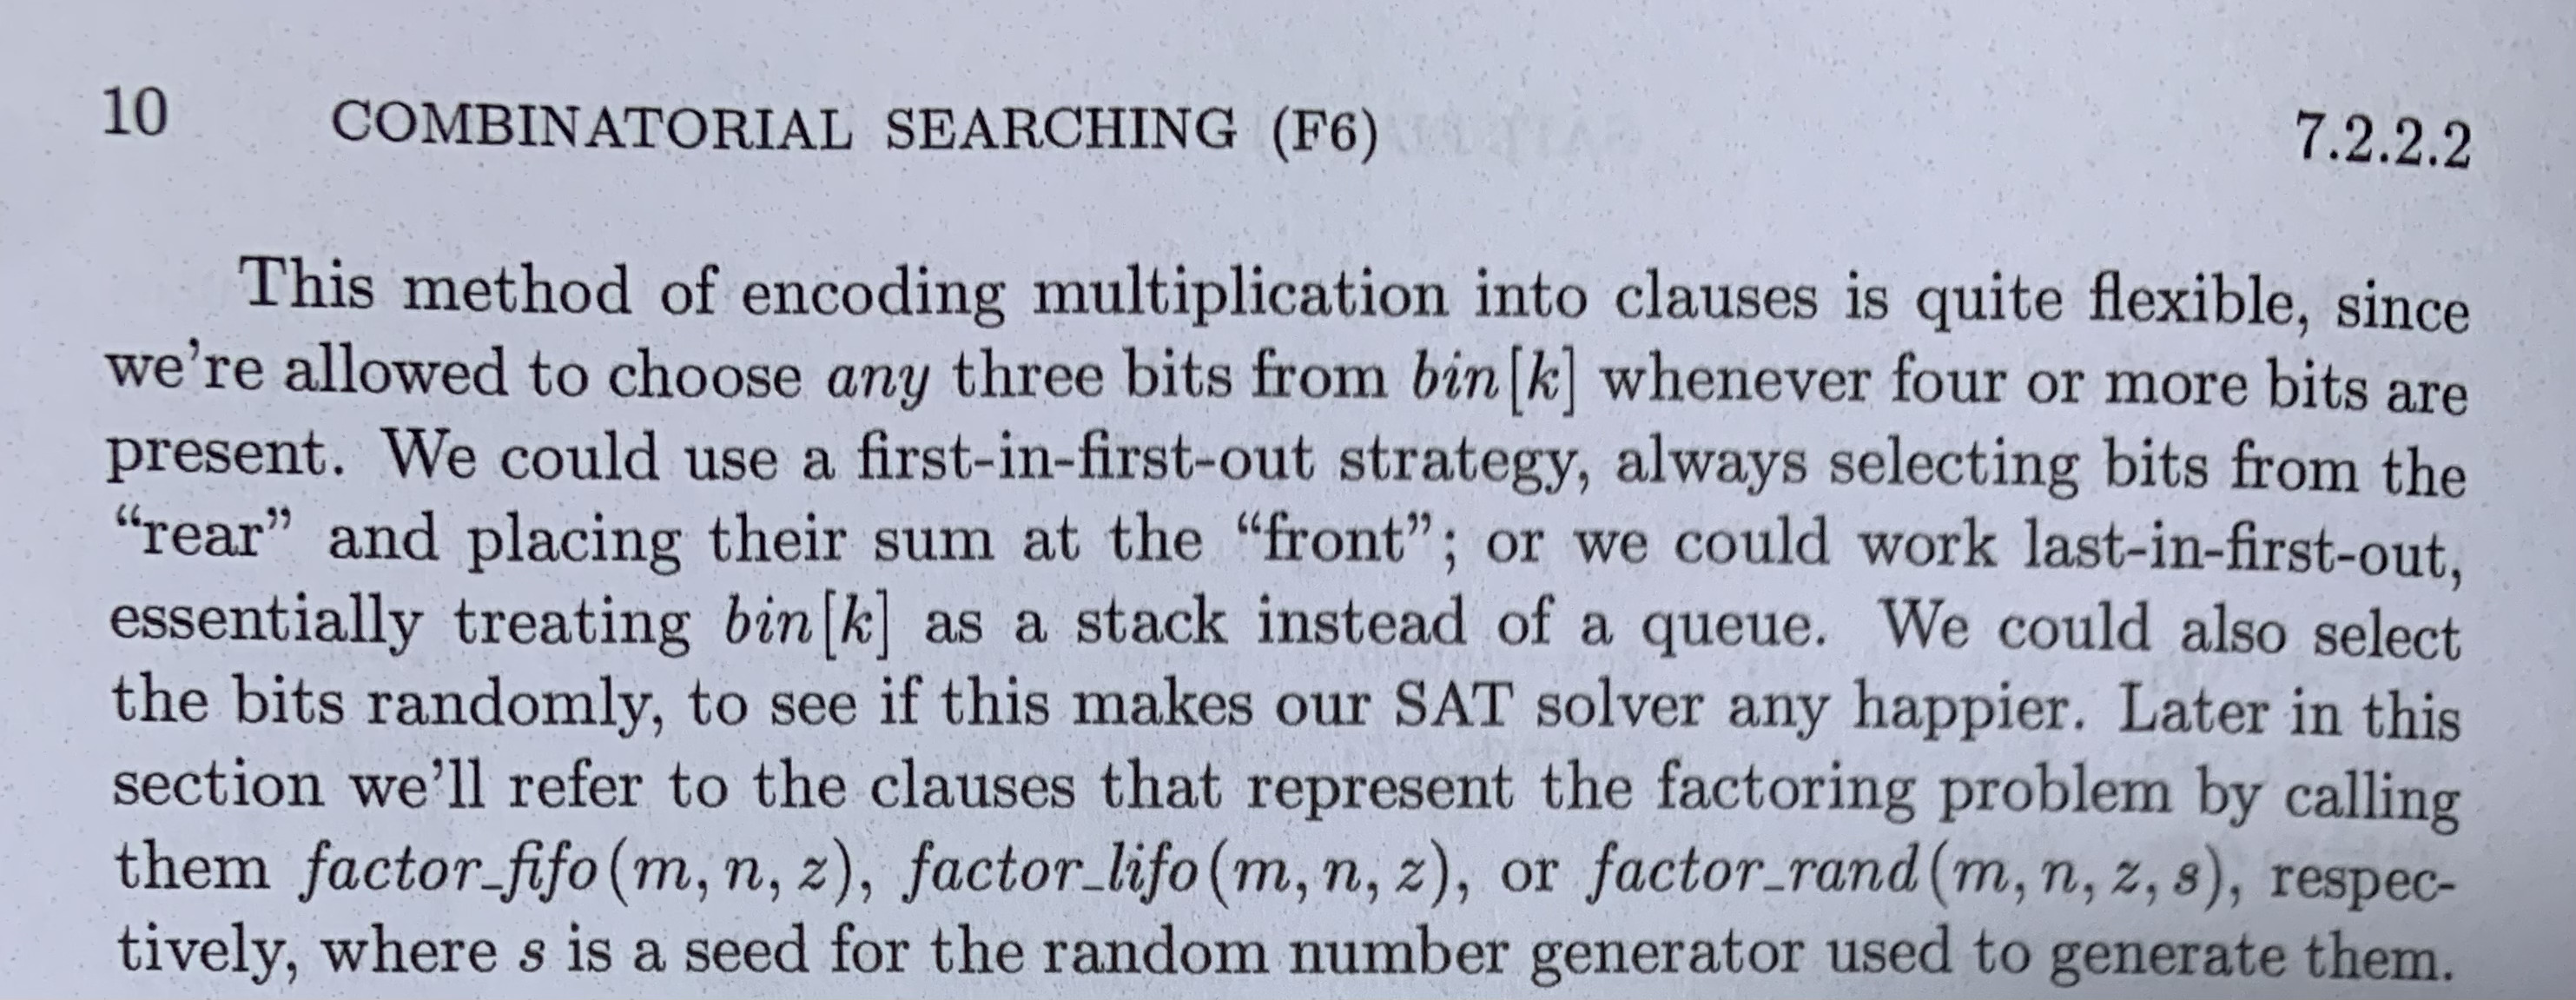
\includegraphics[width=130mm]{images/IMG_7381.jpg}
\end{figure}

乗算を節に符号化するこの方法は非常に柔軟である.我々はbin[k]からどの3ビットでも選択することができるから.4つや,それ以上のビットが存在するときでも.我々は先入れ先出しの戦略を使うことができた,常に"後ろ"からビットを選択し,その和を"前"に配置する; あるいは,後入れ先出しで動作させ,実質的にbin[k]をキューではなくスタックとして扱うこともできた.\footnote{キューは最初に入れたデータを最初に取り出し(FIFO),スタックは最後に入れたデータを最初に取り出す(LIFO)データの取り出し手順}また,ビットをランダムに選択し,それが我々のSATソルバーをより幸せにするかどうかを確認することもできる.このセクションの後半では、因数分解問題を表す節について参照する,それぞれ$factor\_fifo(m,n,z)$, $factor\_lifo(m,n,z)$, $factor\_rand(m,n,z,s)$と呼び,$s$は生成に使用する乱数ジェネレーターのシードであるとする.
%%%%%%%%%%%%%%%%%%%%%%%%%
\newpage
\begin{figure}[htbp]
  \centering
  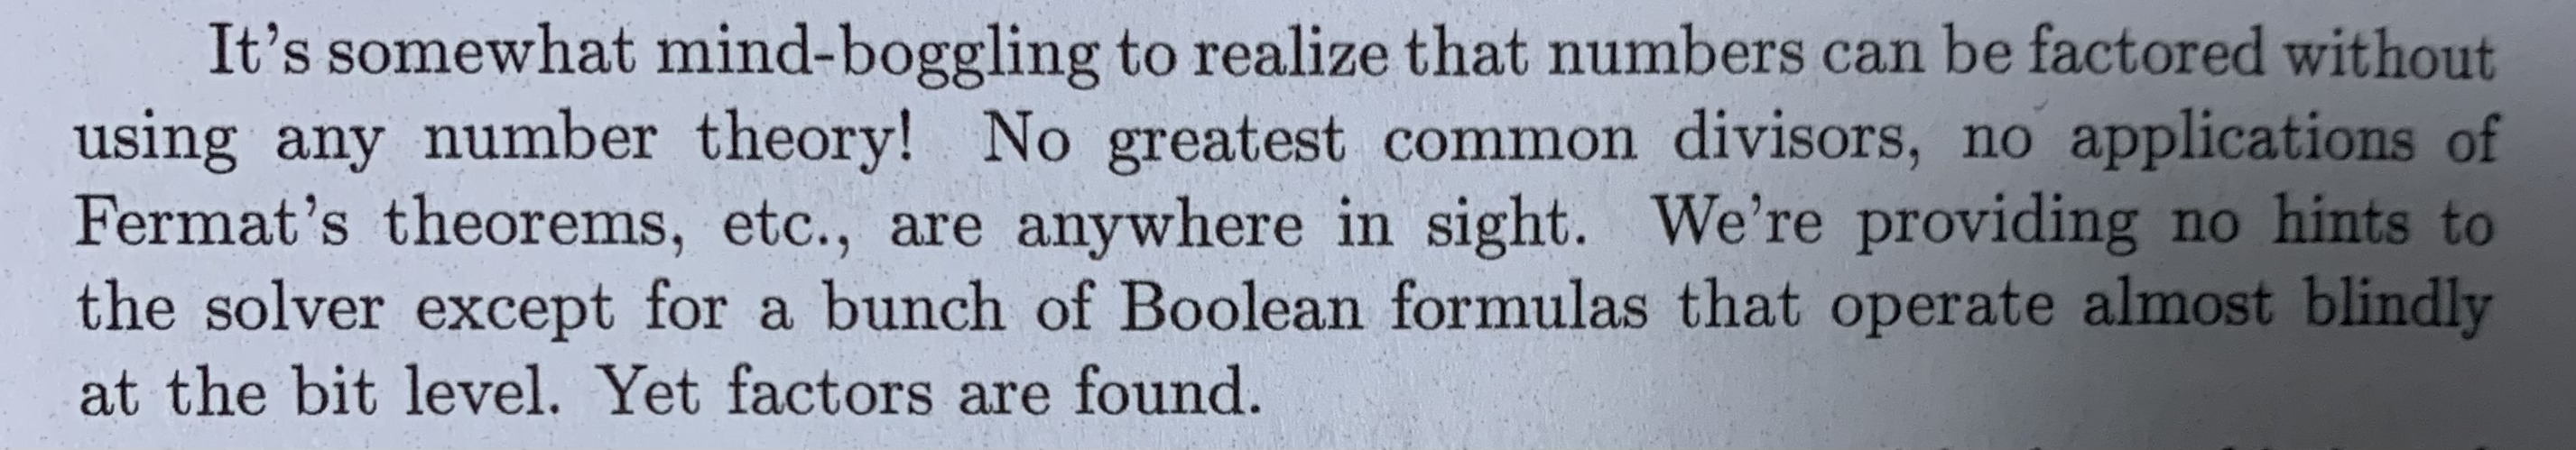
\includegraphics[width=130mm]{images/IMG_73812.jpg}
\end{figure}
数字を何の数論も用いずに因数分解できることに,幾分驚かされる!最大公約数もなければ,フェルマーの定理の応用もなく,他にも何もない...,それらはどこにでもあるようなものである.我々はSATソルバーへのヒントは全く与えていない
ブール式の束を除いて,ビットレベルでほとんど盲目的に動作する.それでも因数は見つかる.
\begin{figure}[htbp]
  \centering
  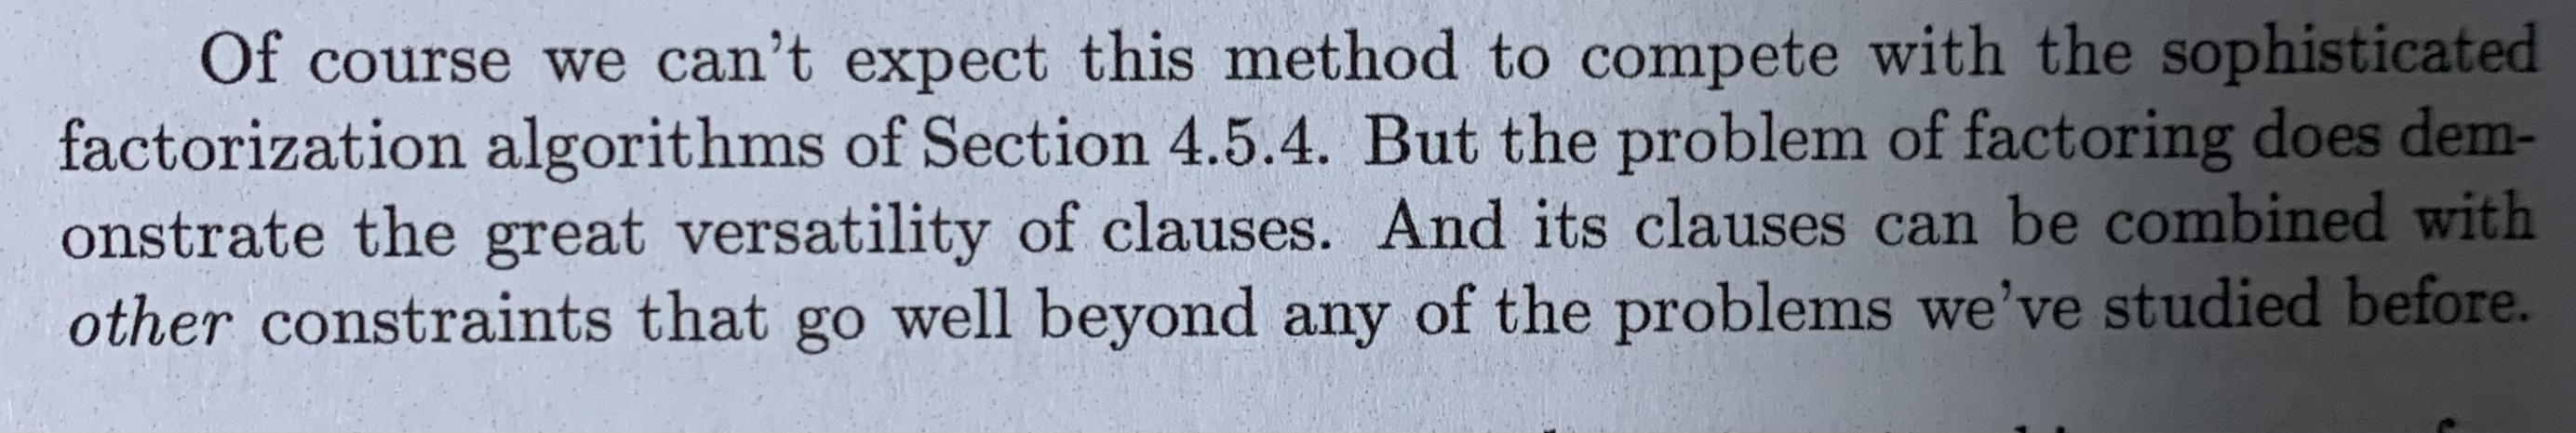
\includegraphics[width=130mm]{images/IMG_73813.jpg}
  \end{figure}

  もちろん,我々は予期できない,この方法が4.5.4節の高度な因数分解アルゴリズムと競合することを.しかし,因数分解の問題は,節の素晴らしい汎用性を示している.そしてそれらの節は他の制約と組み合わせることができ,我々がこれまで研究してきたどの問題よりもはるかに優れている.


%%%%%%%%%%%%%%%%%%%%%%%%%
\newpage
\begin{figure}[htbp]
  \centering
  
\includegraphics[width=130mm]{images/e1.jpeg}
\end{figure}
Ex41.ブール演算子$\wedge ,\vee ,\oplus$の数を決定せよ.Daddaの方式でmビットの数をnビット数で乗算するのに必要な,$2 \leq m \leq n$のとき.

\begin{figure}[htbp]
  \centering
  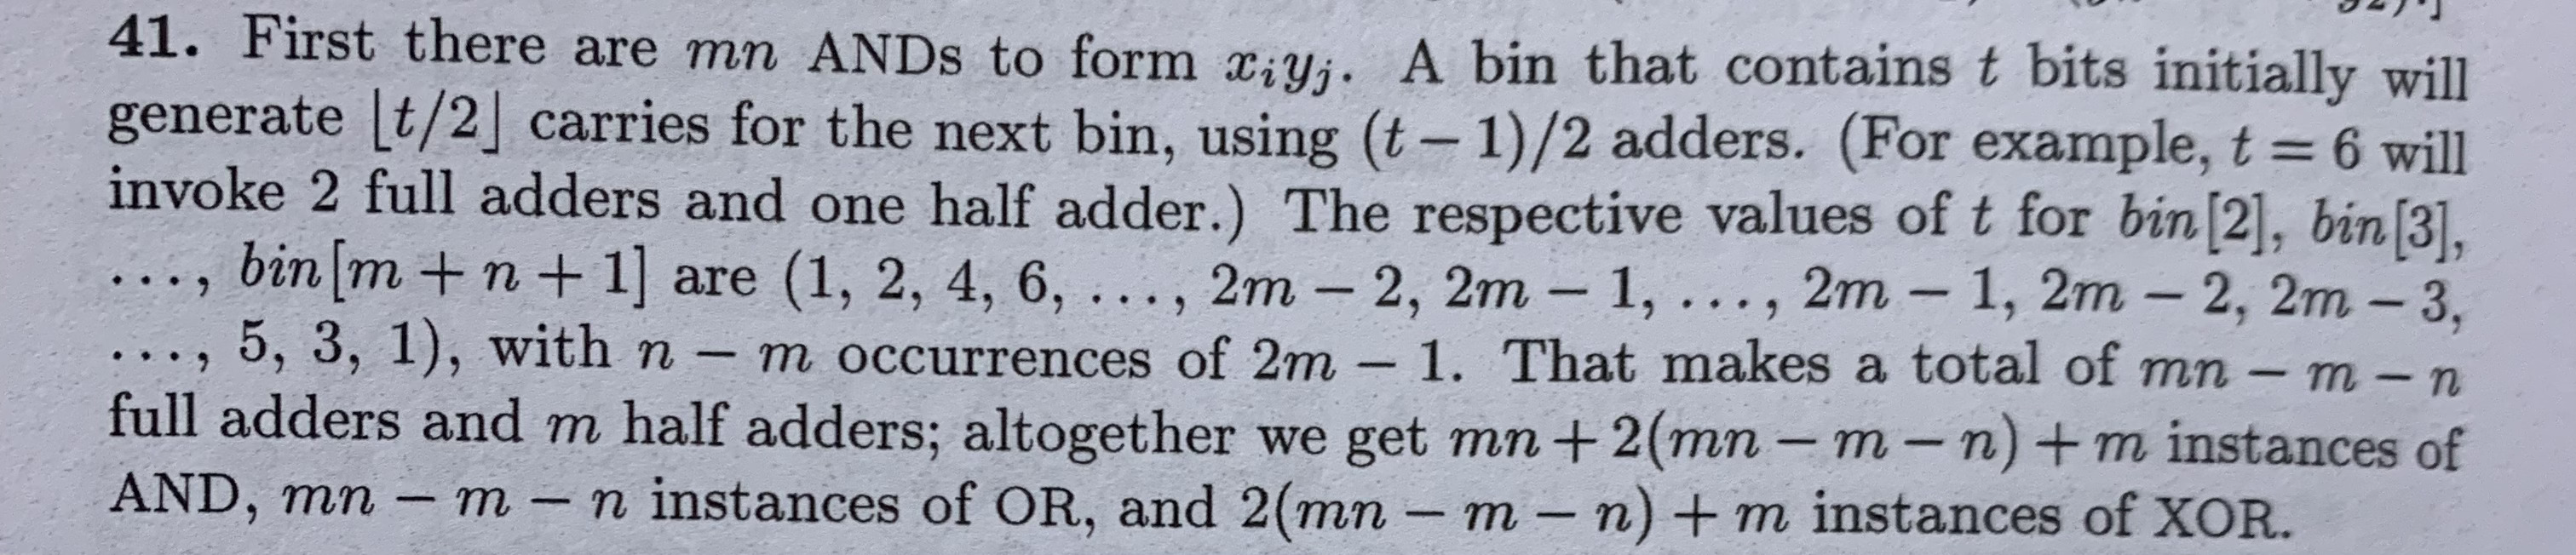
\includegraphics[width=130mm]{images/e2.jpg}
\end{figure}

まず、$x_{i}y_{j}$を形成するために$mn$個のANDがある.
t個のビットを含むbinは最初に,次のbinのために$\lfloor t/2 \rfloor $個のキャリーを生成する,$(t-1)/2$個の加算器を使って.\footnote{ここで言うaddersは全加算器のこと}(例えば,t = 6の場合2つの全加算器と1つの半加算器を呼び出す)\footnote{全加算器は下からの繰り上がりを考慮し,3つを加算するもの,半加算器は2つを加算するもの} \footnote{即ちt=6の場合,(i)3つ選んで全加算器で計算(tが4になる) (ii)3つ選んで全加算器で計算(tが2になる) (iii)残り2つを半加算器で計算となる}
bin[2],bin[3]、...,bin[m+n+1]のそれぞれのtの値は,(1,2,4,6,...,2m-2,2m-1,...,2m-1,2m-2,2m-3,...,5,3,1)となり,2m-1はn-m回発生する.
 それは合計mn-m-nの全加算器とmの半加算器を作り,併せてmn+2(mn-m-n)+m個のANDのインスタンスと,mn-m-nのORのインスタンスと,2(mn-m-n)+mのXORのインスタンスを得られる.
\newpage

\begin{figure}[htbp]
  \centering
  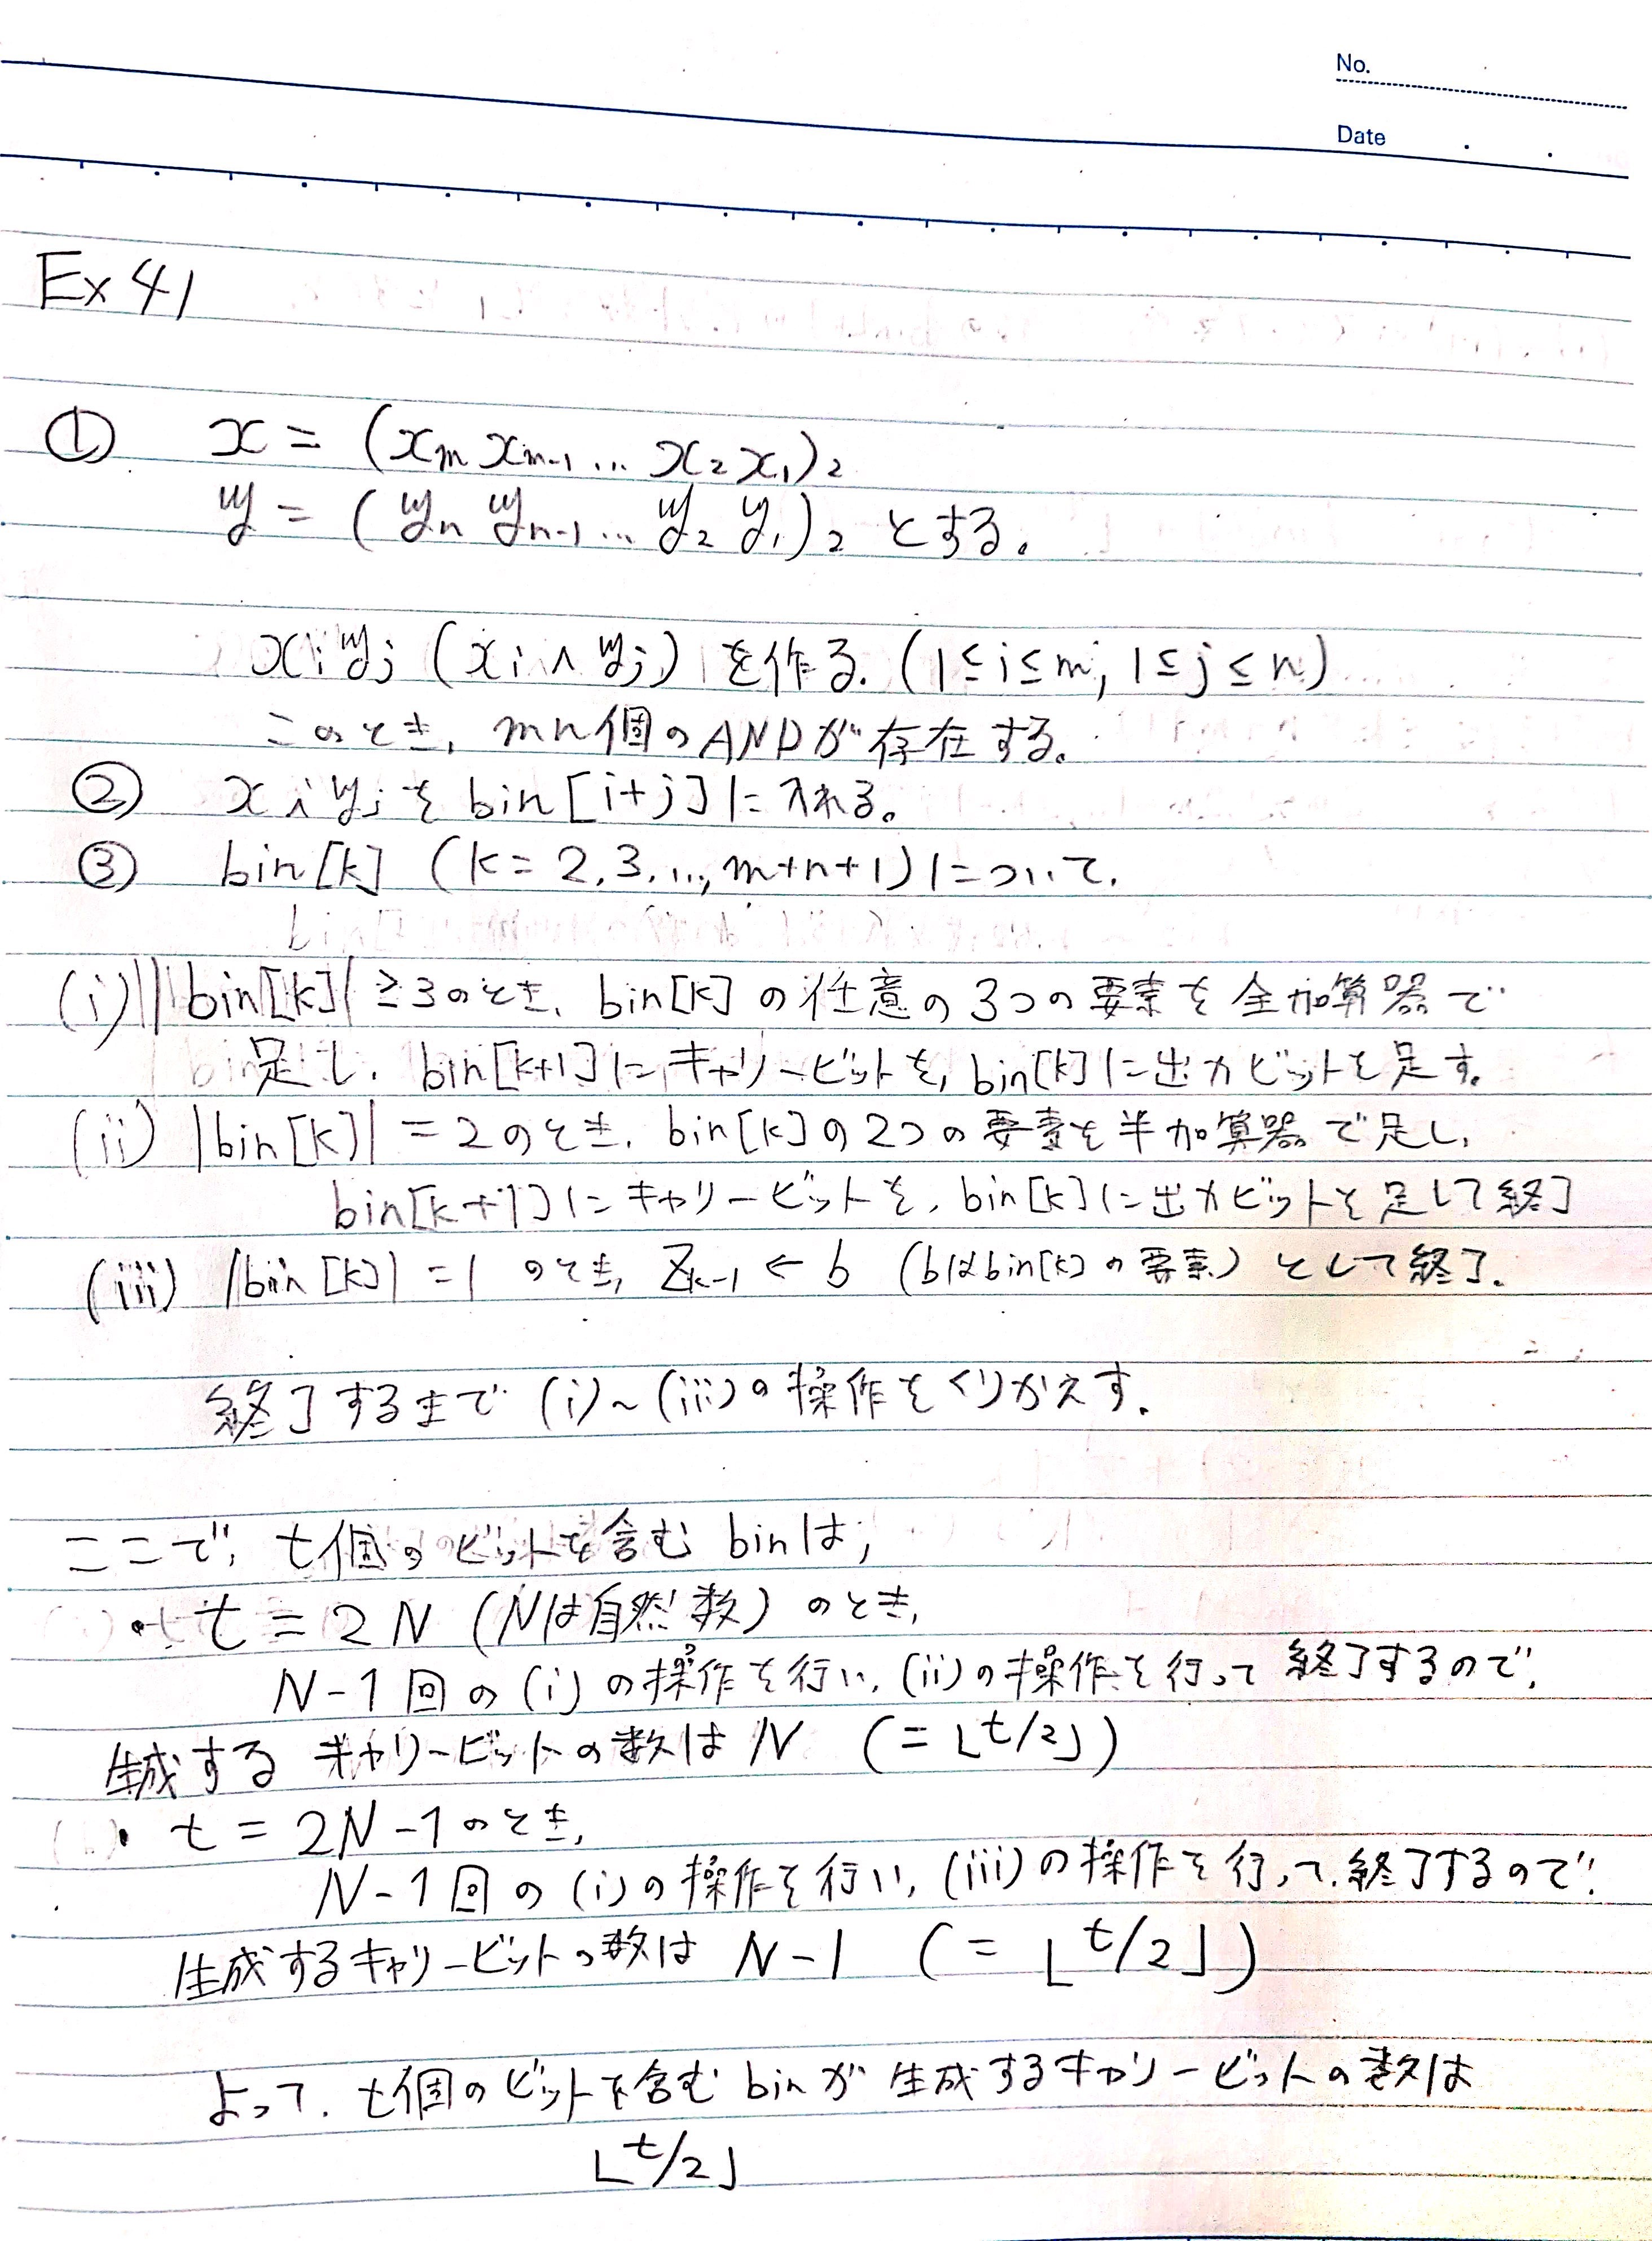
\includegraphics[width=130mm]{images/IMG_7422.JPG}
\end{figure}
\begin{figure}[htbp]
  \centering
  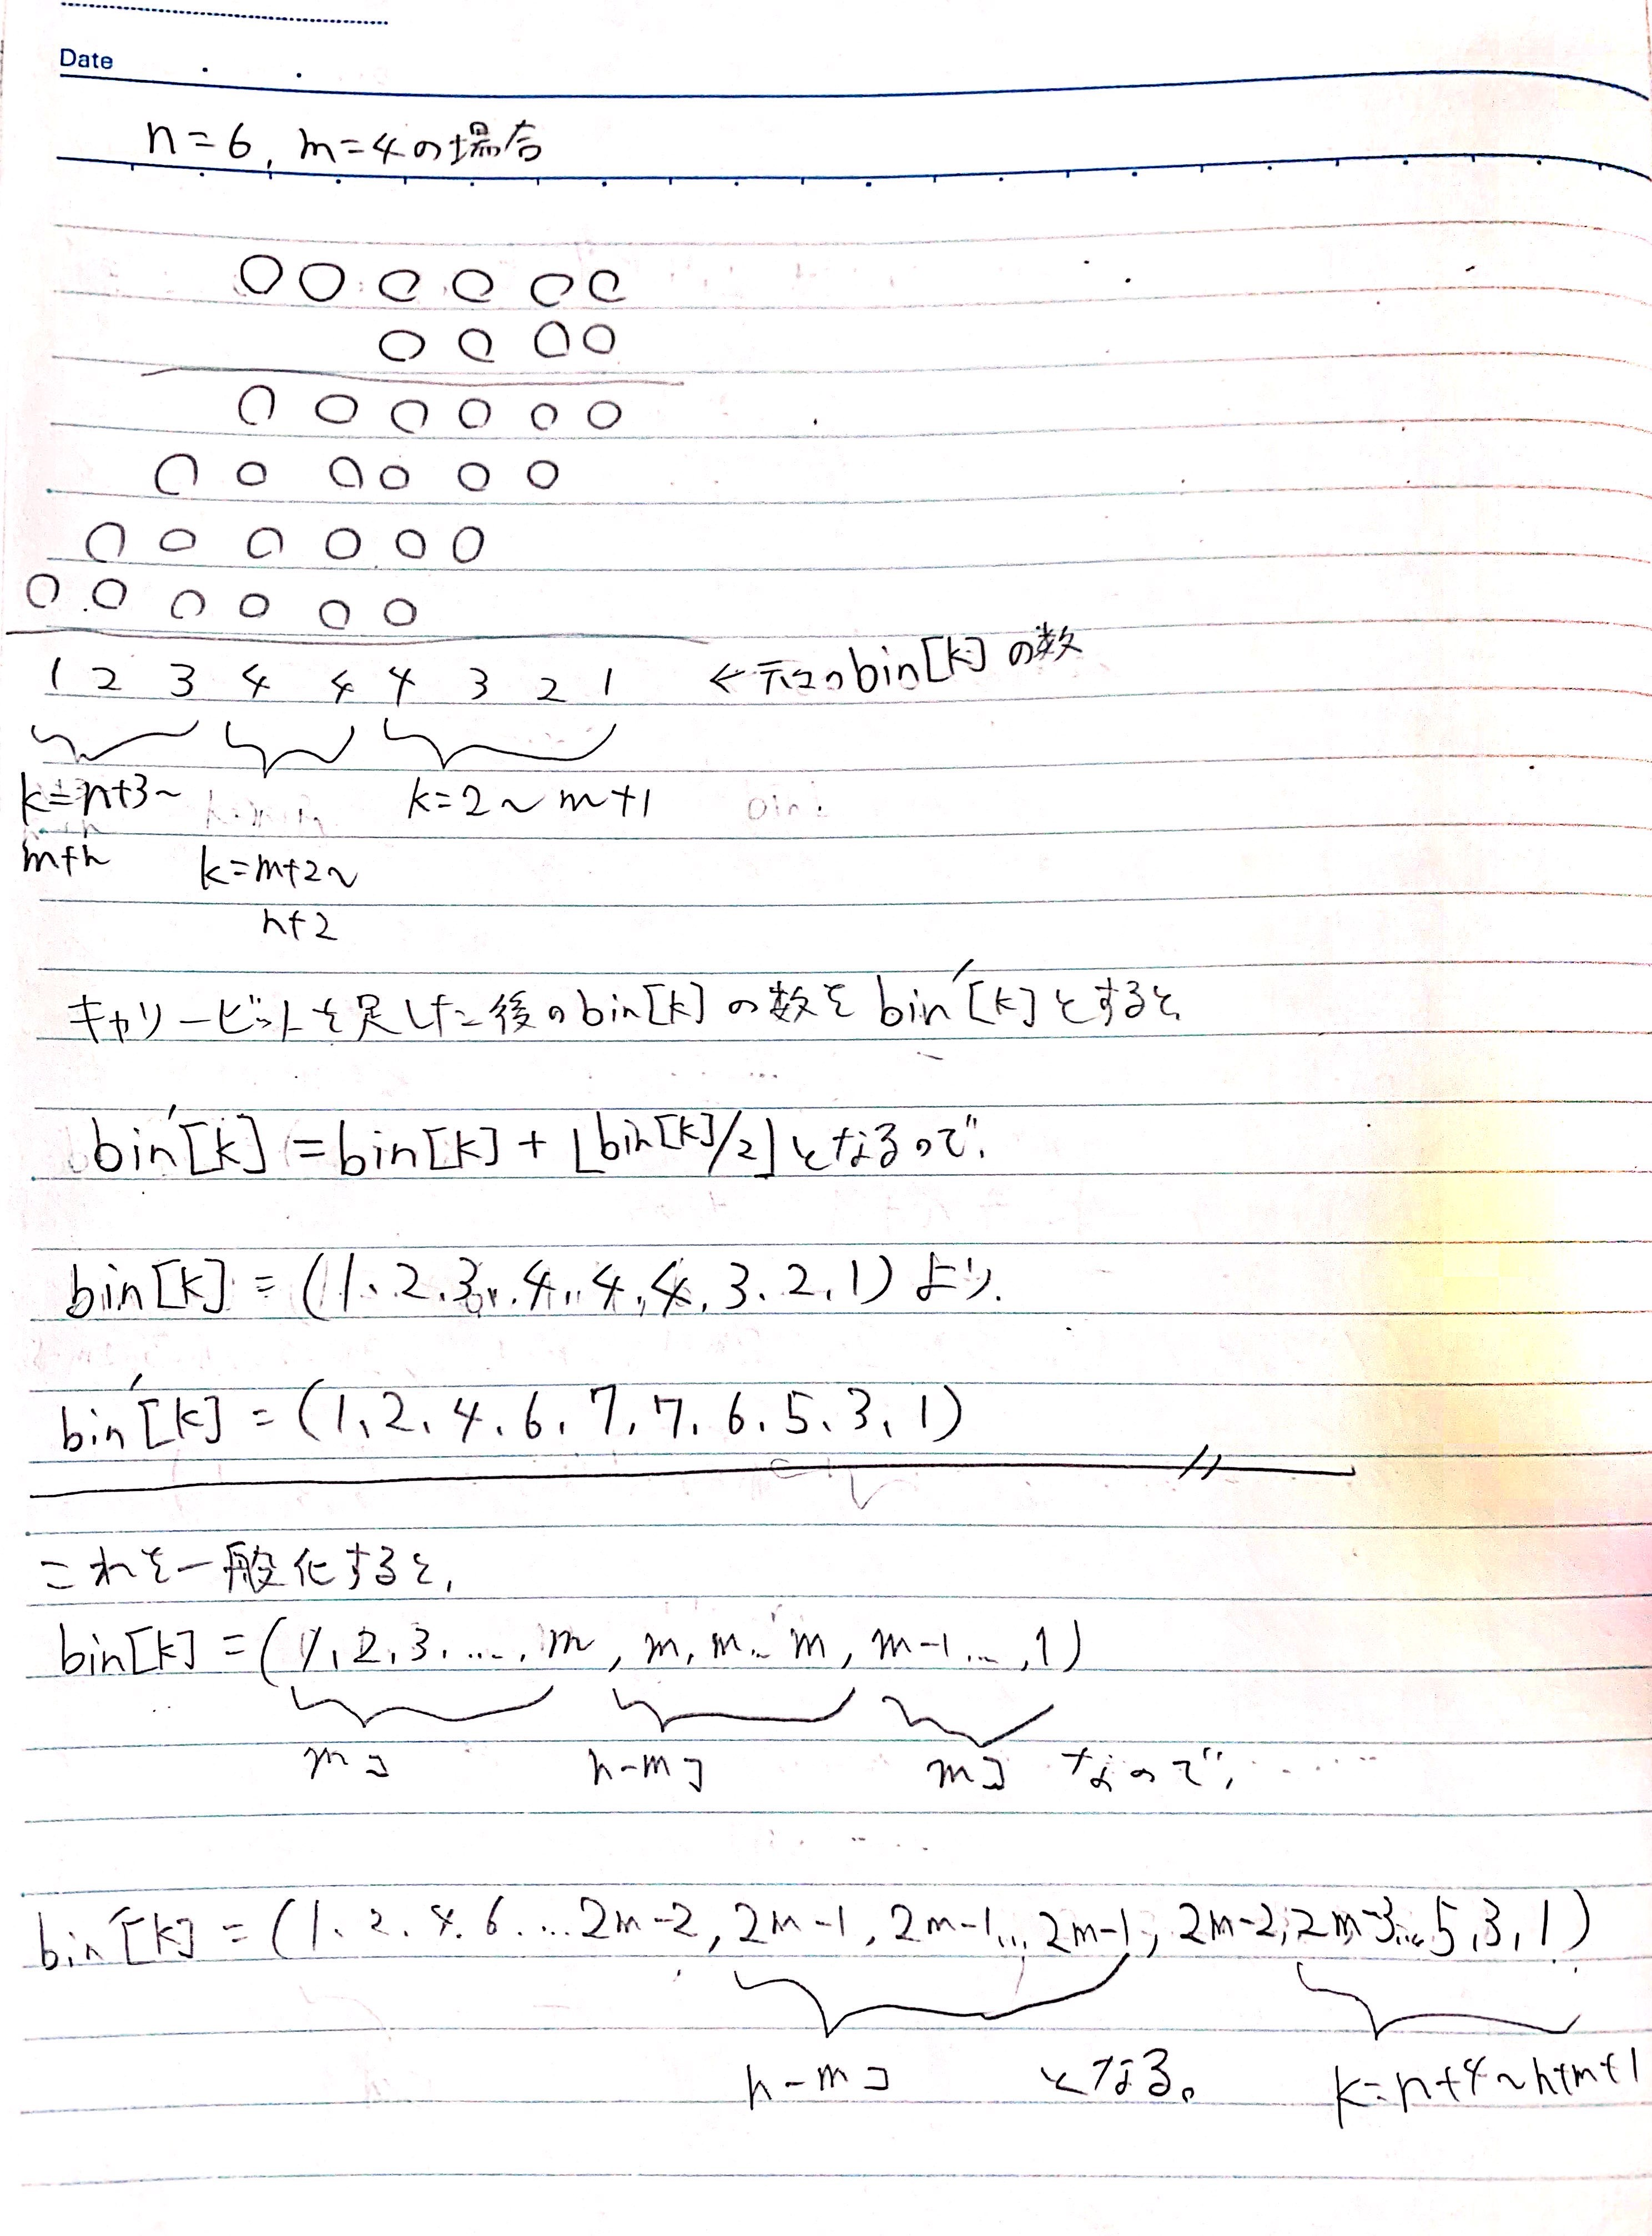
\includegraphics[width=130mm]{images/IMG_7423.JPG}
\end{figure}
\begin{figure}[htbp]
  \centering
  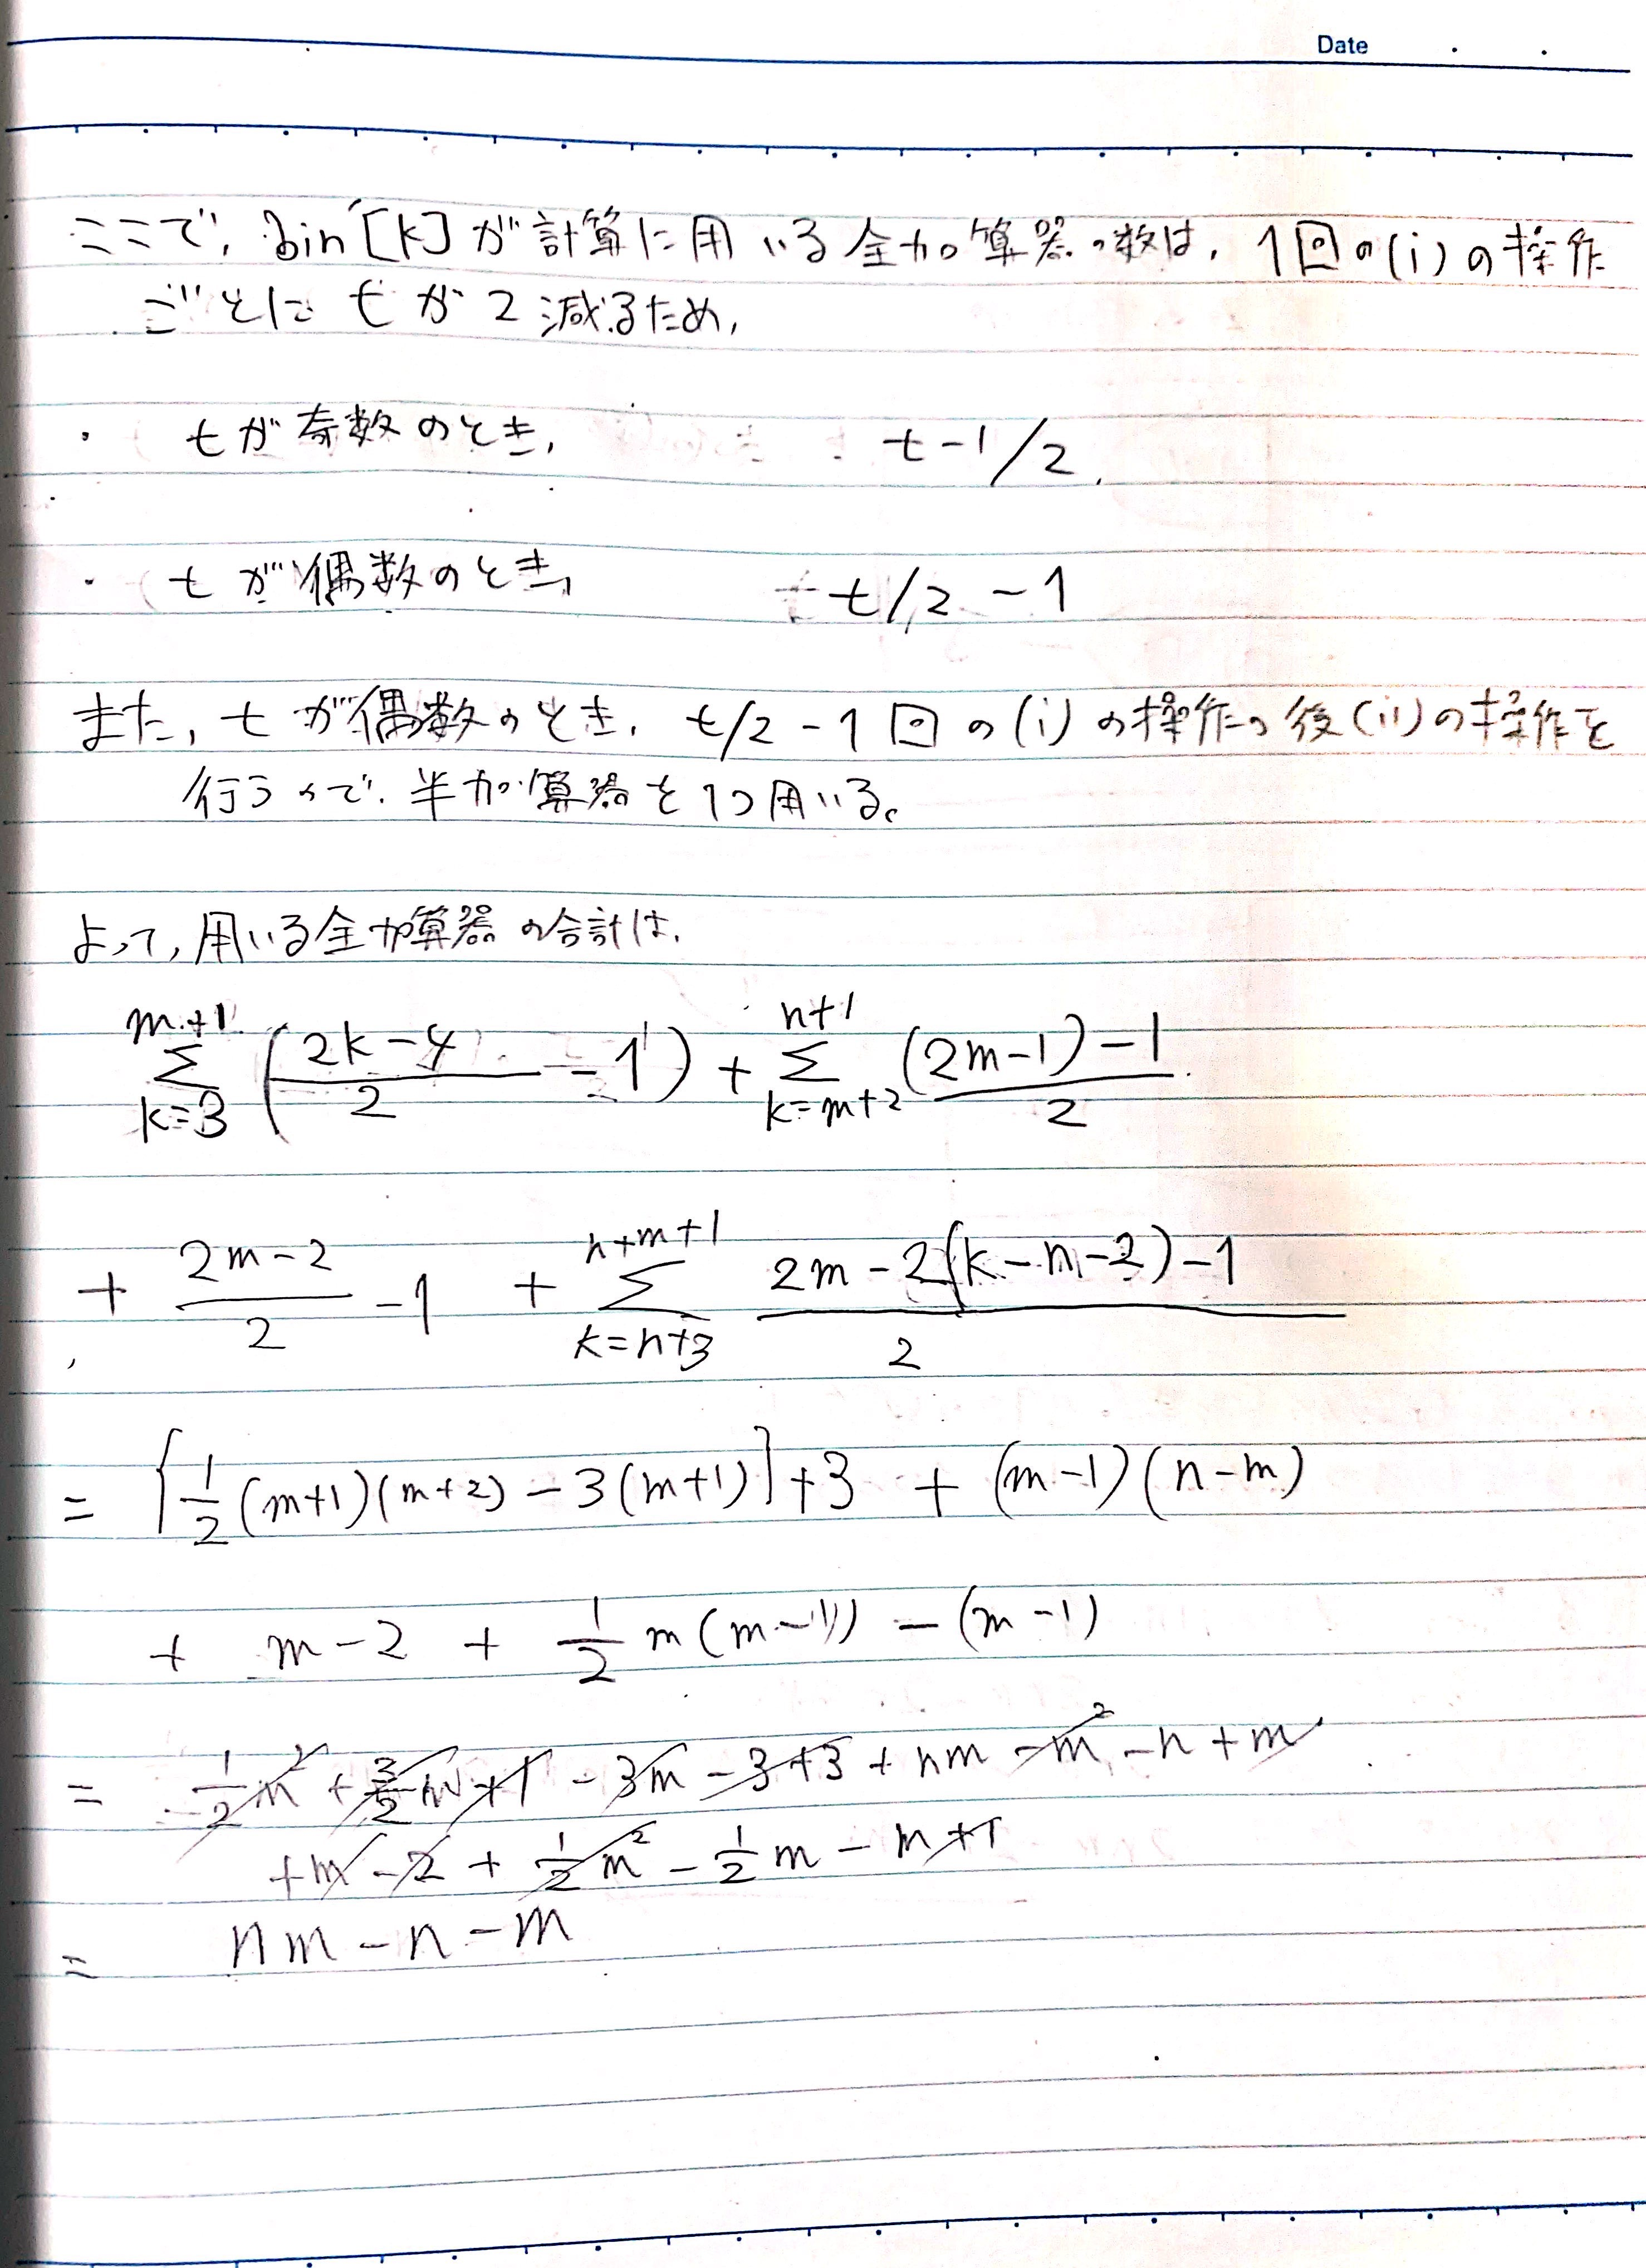
\includegraphics[width=130mm]{images/IMG_7424.JPG}
\end{figure}
\begin{figure}[htbp]
  \centering
  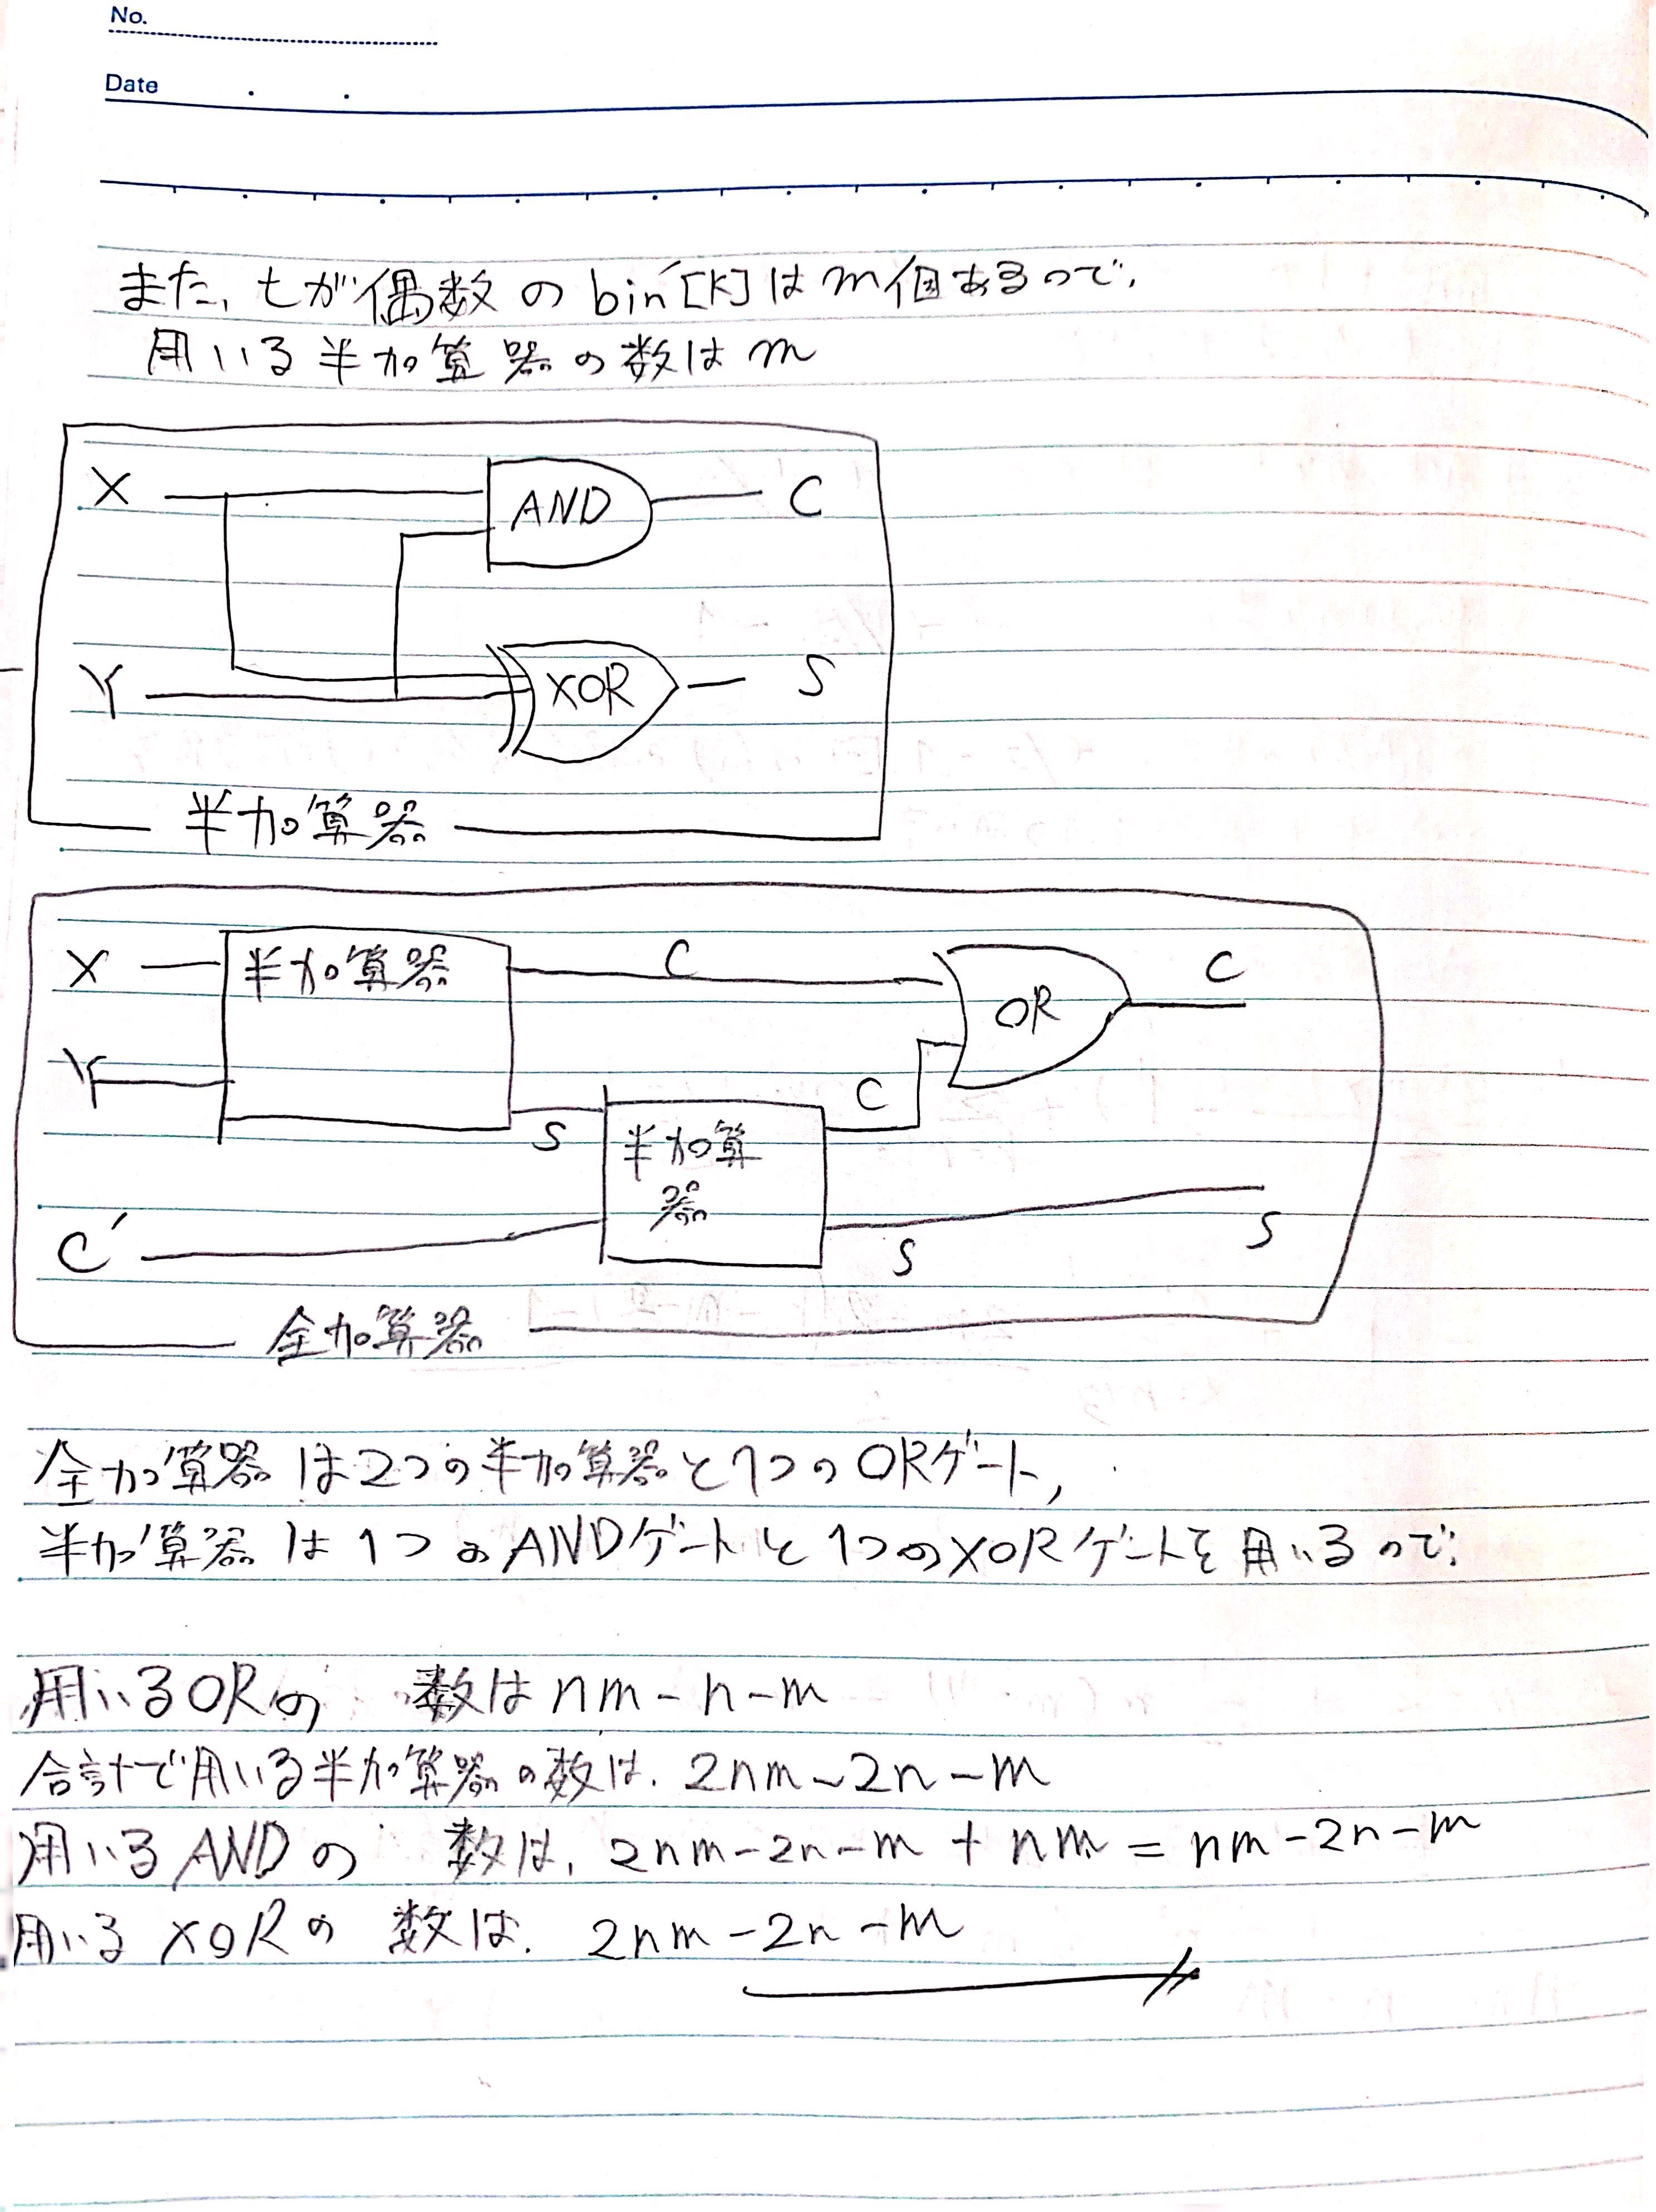
\includegraphics[width=130mm]{images/IMG_7425.JPG}
\end{figure}




 

\end{document}


